\mode*
\mode<all>{\topsection{Geodezyjne II}}
\mode<all>{\midsection{Równania geodezyjnych}}
Dotychczas nie używaliśmy jeszcze lokalnych układów współrzędnych do analizy geodezyjnych. W następującym lemacie pokażemy, że warunek z definicji krzywej geodezyjnej lokalnie wyraża się jako układ równań różniczkowych. Będziemy mogli wtedy użyć ogólnych twierdzeń o rozwiązaniach tych układów, aby dać pewne warunki przy których geodezyjne istnieją i są jednoznaczne.

\begin{frame}

\mode<article>{\begin{twierdzenie}[Równania geodezyjnych]
Niech $M\subset \R^3$ będzie powierzchnią gładką i niech $x\colon U\to M\subset \R^3$ będzie lokalnym układem współrzędnych. Niech $\gamma\colon (a, b)\to x(U)\subset M$ będzie krzywą gładką. Oznaczmy przez
\begin{align*}
g\define x^{-1}\circ\gamma\colon (a,b)&\to U\subset \R^2\\
t&\mapsto (g_1(t),g_2(t))
\end{align*}
i niech $g_1$, $g_2$ będą funkcjami współrzędnych $g(t)$. Pochodna kowariantna krzywej $\gamma$ wyraża się jako
\[\frac{\widehat{D}\gamma'}{dt}=\sum_{k=1}^2\left(g_{k}''(t)+\sum_{i=1}^2\sum_{j=1}^2\Gamma_{ij}^k(g(t))g_i'(t)g_{j}'(t)\right) x_k(g(t).\]
Stąd wynika, że $\gamma$ jest krzywą geodezyjną wtedy i tylko wtedy, gdy te współczynniki są zerowe, tj. spełnione są następujące równania:
\[
\le\{\begin{aligned}
g''_1+\Gamma^1_{11}(g'_1)^2+2\Gamma^1_{12}g'_1g'_2+\Gamma^1_{22}(g'_2)^2&=0\\
g''_2+\Gamma^2_{11}(g'_1)^2+2\Gamma^2_{12}g'_1g'_2+\Gamma^2_{22}(g'_2)^2&=0
\end{aligned}\ri.\]
\end{twierdzenie}}


\mode<presentation>{\begin{twierdzenie}
Niech $M\subset \R^3$ będzie powierzchnią gładką i niech $x\colon U\to M\subset \R^3$ będzie lokalnym układem współrzędnych. Niech $\gamma\colon (a, b)\to x(U)\subset M$ będzie krzywą gładką. \pause Oznaczmy przez
\begin{align*}
g\define x^{-1}\circ\gamma\colon (a,b)&\to U\subset \R^2\\
t&\mapsto (g_1(t),g_2(t))
\end{align*}
i niech $g_1$, $g_2$ będą funkcjami współrzędnych $g(t)$. \pause Pochodna kowariantna krzywej $\gamma$ wyraża się jako
\[\frac{\widehat{D}\gamma'}{dt}=\sum_{k=1}^2\left(g_{k}''(t)+\sum_{i=1}^2\sum_{j=1}^2\Gamma_{ij}^k(g(t))g_i'(t)g_{j}'(t)\right) x_k(g(t).\]
\end{twierdzenie}}

\end{frame}
%%%%%%next-slide%%%%%
\begin{frame}


\mode<presentation>{\begin{wniosek}[Równania geodezyjnych]
Krzywa $\gamma$ jest geodezyjną wtedy i tylko wtedy, gdy te współczynniki są zerowe, tj. spełnione są następujące równania:
\[
\le\{\begin{aligned}
g''_1+\Gamma^1_{11}(g'_1)^2+2\Gamma^1_{12}g'_1g'_2+\Gamma^1_{22}(g'_2)^2&=0\\
g''_2+\Gamma^2_{11}(g'_1)^2+2\Gamma^2_{12}g'_1g'_2+\Gamma^2_{22}(g'_2)^2&=0
\end{aligned}\ri.\]
\end{wniosek}}
\pause 
\mode<presentation>{Dowód twierdzenia i wniosku jest długi i dosyć techniczny, więc na wykładzie go pominiemy. Skupimy się natomiast na przykładzie powierzchni obrotowej.}
\end{frame}
%%%%%%next-slide%%%%%

Dowód jest dosyć techniczny, jednak polega tylko na bezpośrednim przeliczeniu powyższej pochodnej kowariantnej. Można go potraktować jako ćwiczenie na zrozumienie definicji pochodnej pola wektorowego. Dla ułatwienia orientacji wszystkie krzywe $\R\to U\subset \R^2$ nazywamy literami łacińskimi, zaś krzywe $\R\to M\subset\R^3$ -- greckimi.


\textcolor{ared}{\textbf{Dowód:}}\\
Musimy wyrazić równość $\frac{\widehat{D}\gamma'}{dt}=0$ w terminach lokalnego układu współrzędnych. 
Zauważmy, że pole wektorów stycznych do $\gamma$ wyraża się w bazie $\{x_1,x_2\}$ następująco:\[\gamma'(t)=(x\circ g)'(t)=x_1(g(t))g_1'(t)+x_2(g(t))g_2'(t).\]
\begin{itemize}
\item Spróbujmy policzyć bezpośrednio pochodną stycznego pola wektorowego.
\begin{multline}\label{eqn:loc-geod}
\frac{\widehat{D}\gamma'}{dt}=\sum_{i=1}^2 \frac{\widehat{D}}{dt}\left[g_1'(t) x_i(g(t))\right]=\\
=\sum_{i=1}^2\left(\frac{d g_i'(t)}{dt}x_i(g(t))+g_i'(t)\frac{\widehat{D}(x_{i}\circ g)}{dt}(t)\right)
\end{multline}

\item Aby kontynuować musimy zbadać krzywą $x_i\circ g=(x_i\circ x^{-1})\circ \gamma$ i policzyć jej pochodną
kowariantną. W poniższych rachunkach będziemy pomijać argumenty funkcji, należy zatem pamiętać, że wszystko dzieje się w punkcie $g(t)$.}

\item Mamy następującą równość:
\begin{multline*}
\frac{\widehat{D}(x_i\circ g)}{dt}(t)=
\Pi_{T_{\gamma(t)}M}\le(\frac{d\left((x_i\circ x^{-1})\circ \gamma\right)}{dt}(t)\ri)=\\ =\widehat{\nabla}_{\gamma'(t)}\le(x_i\circ x^{-1}\ri)=\widehat{\nabla}_{\left[x_1(g(t))g_1'(t)+x_2(g(t))g_2'(t)\right]}x_i=\\
=g_1'(t)\widehat{\nabla}_{x_1(g(t))}\le(x_i\circ x^{-1}\ri)+g_2'(t)\widehat{\nabla}_{x_2(g(t))}\le(x_i\circ x^{-1}\ri).
\end{multline*}
Skorzystaliśmy tutaj z liniowości pochodnej kowariantnej. 

\item Niech $a^{1}\colon (-\varepsilon,\varepsilon)\to U$ będzie krzywą zadaną wzorem
\[a^{1}(s)=\define(s+g_1(t),g_2(t)).\] Podobnie można zdefiniować $a^{2}$. Wtedy (sprawdzić!)
\begin{multline*}
\widehat{\nabla}_{x_1(g(t))}\le(x_i\circ x^{-1}\ri)=\Pi_{T_{\gamma(t)}M}\le(\frac{d\le( x_i\circ x^{-1}\circ x\circ a^{j}\ri)}{ds}\Bigg|_{s=0}\ri)=\\
=\Pi_{T_{\gamma(t)}M}\le(\frac{d\le(x_i\circ a^{j}\ri)}{ds}\Bigg|_{s=0}\ri)=\Pi_{T_{\gamma(t)}M}x_{ij}\le(g(t)\ri)
\end{multline*}

\item Skorzystajmy teraz z formuła Gaussy wyrażającej $x_{ij}$ jako odpowiednią kombinację liniową:
\begin{multline*}
g_1'(t)\Pi_{T_{\gamma(t)}M}\left(x_{1i}(g(t))\right)+g_2'(t)\Pi_{T_{\gamma(t)}M}\left(x_{2i}(g(t))\right)=\\
=c_1'(t)\left(\Gamma_{1i}^1(g(t)) x_1(g(t)) +\Gamma_{1i}^2(g(t)) x_2(g(t)) \right)+\\ +c_2'(t)\left(\Gamma_{2i}^1(g(t)) x_1(g(t)) +\Gamma_{2i}^2(g(t)) x_2(g(t)) \right)
\end{multline*}
%gdzie w ostatnim wierszu wszystkie symbole Christoffela i pochodne $x_i$ są wyewaluowane w punkcie $g(t)$.

\item Grupując odpowiednie wyrazy możemy tę równość zapisać
\[\frac{\widehat{D}(x_i\circ g)}{dt}(t)=\sum_{k=1}^2\sum_{j=1}^2\Gamma^k_{ji}(g(t))g_{j}'(t)x_{k}(g(t)).\]

\item Wstawiając uzyskaną równość do równania \ref{eqn:loc-geod} powyżej otrzymujemy

\[\frac{\widehat{D}\gamma'}{dt}=\sum_{i=1}^2\left(g_i''(t)x_i(g(t))+g_{i}'(t)\sum_{k=1}^2\sum_{j=1}^2\Gamma^k_{ji}(g(t))g_{j}'(t)x_{k}(g(t))\right)\]
%gdzie w ostatniej równości użyliśmy wyprowadzonej przed chwilą formuły.

\item Ponownie zmieniając kolejność sumowania i grupując otrzymujemy
\[\frac{\widehat{D}\gamma'}{dt}=\sum_{k=1}^2\left(g_{k}''(t)+\sum_{i=1}^2\sum_{j=1}^2\Gamma_{ij}^k(g(t))g_i'(t)g_{j}'(t)\right) x_k(g(t),\]
co kończy dowód.
\end{itemize}

\hfill $\square$

%%%%%%next-slide%%%%%
\mode<all>{\lowsection{Przykład: powierzchnia obrotowa}}

\begin{frame}[<+->]{Przykład: powierzchnia obrotowa}
\begin{wniosek}
Niech $M\subset \R^3$ będzie powierzchnią obrotową z lokalnym układem współrzędnych
\[x(t,\vartheta)=(\alpha_1(t),\alpha_2(t)\cos(\vartheta),\alpha_2(t)\sin(\vartheta)),\]
oraz załóżmy, że krzywa profilu $x(t,0)=(\alpha_1(t),\alpha_2(t),0)$ jest unormowana. Wtedy 
\begin{enumerate}
\item Każda krzywa profilu (południk) na powierzchni $M$ może być sparametryzowana jako krzywa geodezyjna.
\item Okrąg na powierzchni $M$ prostopadły do osi obrotu (równoleżnik) może być sparametryzowany jako krzywa geodezyjna wtedy i tylko wtedy, gdy wektor styczny do krzywej profilu w punkcie przecięcia z z tym równoleżnikiem jest równoległy do osi obrotu.
\end{enumerate}
\end{wniosek}

\end{frame}
%%%%%%next-slide%%%%%
\begin{frame}

\begin{center}

\definecolor{c000080}{RGB}{0,0,128}
\definecolor{c800080}{RGB}{128,0,128}
\definecolor{c808080}{RGB}{128,128,128}
\definecolor{c0000ff}{RGB}{0,0,255}
\definecolor{cff0000}{RGB}{255,0,0}
\usetikzlibrary{arrows}

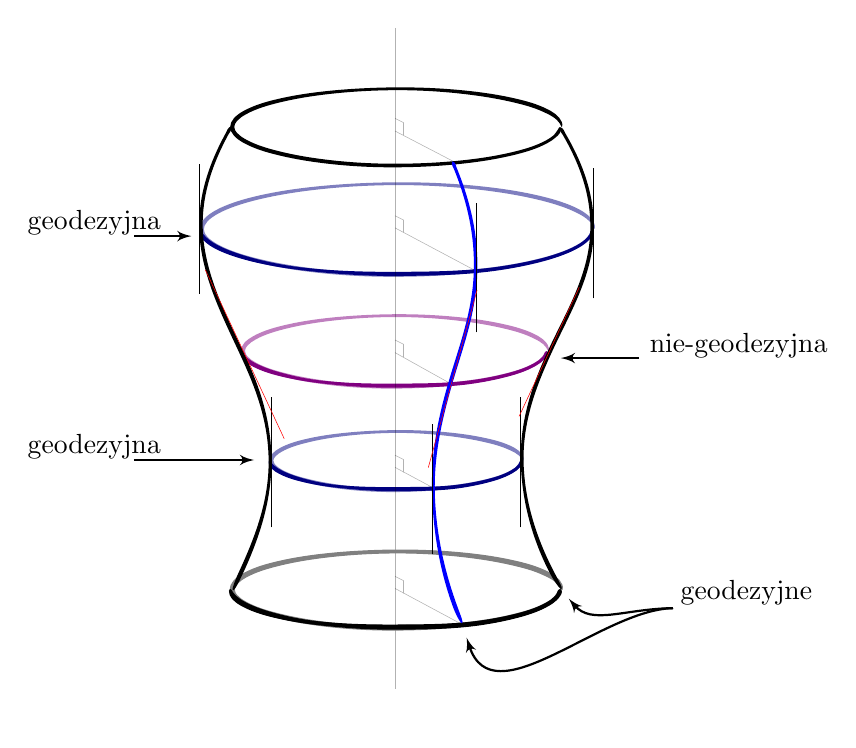
\begin{tikzpicture}[y=0.80pt, x=0.8pt,yscale=-1,scale=0.55, inner sep=0pt, outer sep=0pt]
\begin{scope}[shift={(-54.17497,-482.32144)}]% layer1
  \begin{scope}% g925
    % path1674
    \path[fill=c000080,opacity=0.500] (450.7866,827.3012) .. controls
      (450.3283,827.0404) and (449.8684,826.7940) .. (449.4098,826.5594) .. controls
      (449.4098,826.5594) and (449.4098,826.5594) .. (449.4098,826.5594) .. controls
      (442.1869,822.8104) and (434.3784,820.7957) .. (426.7046,819.1259) .. controls
      (426.7046,819.1259) and (426.7046,819.1259) .. (426.7046,819.1259) .. controls
      (415.8058,816.7341) and (404.7553,815.2537) .. (393.6971,814.2316) .. controls
      (380.3131,812.9930) and (366.8687,812.4733) .. (353.4360,812.5816) .. controls
      (351.2026,812.5995) and (348.9690,812.6348) .. (346.7357,812.6884) .. controls
      (335.5467,812.9575) and (324.3625,813.5575) .. (313.2144,814.6340) .. controls
      (313.2144,814.6340) and (313.2144,814.6340) .. (313.2144,814.6340) .. controls
      (302.1780,815.6988) and (291.1463,817.1973) .. (280.2932,819.6689) .. controls
      (280.2932,819.6689) and (280.2932,819.6689) .. (280.2932,819.6689) .. controls
      (272.6512,821.3996) and (264.9059,823.4939) .. (257.8814,827.3255) .. controls
      (257.8814,827.3255) and (257.8814,827.3255) .. (257.8814,827.3255) .. controls
      (255.6188,828.5492) and (253.3663,830.0341) .. (251.5499,832.0744) .. controls
      (250.2126,833.5415) and (249.2060,835.4962) .. (249.1650,837.6951) .. controls
      (249.1874,838.5732) and (249.3636,839.4101) .. (249.6527,840.1909) .. controls
      (250.0875,841.3653) and (250.7759,842.4140) .. (251.5803,843.2889) .. controls
      (253.4014,845.3151) and (255.6492,846.7911) .. (257.9074,848.0172) .. controls
      (264.9180,851.8550) and (272.6366,854.0333) .. (280.2576,855.8751) .. controls
      (280.2576,855.8751) and (280.2576,855.8751) .. (280.2576,855.8751) .. controls
      (291.0821,858.5061) and (302.1054,860.2255) .. (313.1482,861.4325) .. controls
      (325.7391,862.8104) and (338.4055,863.4823) .. (351.0586,863.4580) .. controls
      (351.8512,863.4560) and (352.6437,863.4530) .. (353.4360,863.4473) .. controls
      (366.8848,863.3526) and (380.3351,862.6708) .. (393.7044,861.2336) .. controls
      (404.7475,860.0477) and (415.7726,858.3772) .. (426.5825,855.7368) .. controls
      (426.5825,855.7368) and (426.5825,855.7368) .. (426.5826,855.7368) .. controls
      (434.1997,853.8857) and (441.9062,851.6679) .. (448.8252,847.7620) .. controls
      (448.8252,847.7620) and (448.8252,847.7620) .. (448.8252,847.7620) .. controls
      (450.5718,846.7821) and (452.3004,845.6555) .. (453.8011,844.2488) .. controls
      (454.2954,843.8922) and (454.7326,843.5155) .. (455.1134,843.1311) .. controls
      (455.8201,842.4296) and (456.3088,841.6591) .. (456.5959,840.9536) .. controls
      (456.8830,840.2482) and (456.9746,839.6092) .. (456.9515,839.1064) .. controls
      (456.9284,838.6036) and (456.7939,838.2358) .. (456.6237,838.0070) .. controls
      (456.4536,837.7782) and (456.2489,837.6859) .. (456.0491,837.6959) .. controls
      (455.6496,837.7159) and (455.2953,838.1099) .. (454.8654,838.6952) .. controls
      (454.4355,839.2806) and (453.8778,840.0946) .. (453.0299,841.2881) .. controls
      (452.7219,841.6985) and (452.3745,842.1410) .. (451.9760,842.6206) .. controls
      (450.7201,843.7471) and (449.2151,844.6997) .. (447.6407,845.5963) .. controls
      (447.6407,845.5963) and (447.6407,845.5963) .. (447.6407,845.5963) .. controls
      (441.0564,849.3040) and (433.5572,851.4015) .. (426.0009,853.2222) .. controls
      (426.0009,853.2222) and (426.0009,853.2222) .. (426.0009,853.2222) .. controls
      (415.3271,855.7789) and (404.4091,857.3770) .. (393.4374,858.5049) .. controls
      (380.1619,859.8684) and (366.8013,860.4813) .. (353.4360,860.5142) .. controls
      (352.8735,860.5152) and (352.3110,860.5162) .. (351.7485,860.5152) .. controls
      (338.9500,860.4992) and (326.1532,859.7677) .. (313.4531,858.3160) .. controls
      (313.4531,858.3160) and (313.4531,858.3160) .. (313.4531,858.3160) .. controls
      (302.5022,857.0632) and (291.6217,855.3187) .. (280.9947,852.6885) .. controls
      (280.9947,852.6885) and (280.9947,852.6885) .. (280.9947,852.6885) .. controls
      (273.4676,850.8107) and (266.0352,848.7138) .. (259.5123,845.0826) .. controls
      (259.5123,845.0826) and (259.5123,845.0826) .. (259.5123,845.0826) .. controls
      (257.4254,843.9026) and (255.4816,842.6611) .. (254.0992,841.0607) .. controls
      (253.8344,840.7353) and (253.5845,840.4030) .. (253.3653,840.0694) .. controls
      (252.8347,839.2619) and (252.4821,838.4435) .. (252.5396,837.6951) .. controls
      (252.4480,836.6464) and (253.1664,835.4379) .. (254.0750,834.3080) .. controls
      (254.0750,834.3080) and (254.0750,834.3080) .. (254.0750,834.3080) .. controls
      (255.4445,832.7025) and (257.3858,831.4454) .. (259.4827,830.2533) .. controls
      (265.9372,826.6389) and (273.3942,824.5274) .. (280.9856,822.6624) .. controls
      (291.6128,820.0721) and (302.5609,818.3858) .. (313.4629,817.1736) .. controls
      (324.8952,815.9036) and (336.2758,815.2010) .. (347.3354,814.9576) .. controls
      (349.3796,814.9126) and (351.4128,814.8878) .. (353.4360,814.8811) .. controls
      (353.4360,814.8811) and (353.4360,814.8811) .. (353.4360,814.8811) .. controls
      (367.1256,814.8369) and (380.3461,815.6201) .. (393.4182,817.0821) .. controls
      (404.3276,818.3034) and (415.1350,819.9482) .. (425.9398,822.4318) .. controls
      (432.6622,823.9886) and (439.4204,825.6818) .. (445.7378,828.5968) .. controls
      (446.3588,828.8737) and (447.0519,829.1866) .. (447.7846,829.5308) .. controls
      (448.8339,830.0287) and (449.9599,830.5787) .. (451.0312,831.1979) .. controls
      (452.1025,831.8170) and (453.1145,832.5109) .. (453.9869,833.2556) .. controls
      (454.7586,833.9204) and (455.4194,834.6415) .. (455.9049,835.3177) .. controls
      (456.3904,835.9940) and (456.7071,836.6271) .. (456.9574,837.0751) .. controls
      (457.2077,837.5231) and (457.4118,837.7842) .. (457.6314,837.6673) .. controls
      (457.8510,837.5504) and (458.1016,837.0388) .. (458.1102,836.0151) .. controls
      (457.9260,834.4159) and (457.1462,832.7521) .. (456.0038,831.4715) .. controls
      (454.5015,829.7196) and (452.5838,828.3523) .. (450.7866,827.3012) -- cycle;

    % path1676
    \path[fill=c000080] (251.1324,844.2113) .. controls (253.0889,846.1463) and
      (255.3435,847.5203) .. (257.5692,848.6355) .. controls (264.7936,852.3040) and
      (272.5617,854.3230) .. (280.2282,856.0022) .. controls (280.2282,856.0022) and
      (280.2282,856.0022) .. (280.2282,856.0022) .. controls (287.3992,857.5841) and
      (294.6432,858.7627) .. (301.9227,859.5839) .. controls (305.6858,860.0085) and
      (309.4502,860.3974) .. (313.2144,860.7555) .. controls (326.5803,862.0281) and
      (340.0067,862.8632) .. (353.4360,862.7487) .. controls (353.4360,862.7487) and
      (353.4360,862.7487) .. (353.4360,862.7487) .. controls (353.7938,862.7457) and
      (354.1515,862.7417) .. (354.5092,862.7375) .. controls (367.5772,862.5769) and
      (380.6754,862.6019) .. (393.7345,861.5412) .. controls (398.2316,861.1766) and
      (402.7273,860.6883) .. (407.1961,859.9991) .. controls (413.7379,858.9902) and
      (420.2454,857.7324) .. (426.6713,856.1203) .. controls (426.6713,856.1203) and
      (426.6713,856.1203) .. (426.6713,856.1203) .. controls (434.2889,854.2215) and
      (442.0142,851.9218) .. (448.9125,847.9216) .. controls (448.9125,847.9216) and
      (448.9125,847.9216) .. (448.9125,847.9216) .. controls (451.1354,846.6419) and
      (453.3307,845.1117) .. (455.0476,843.0728) .. controls (455.0476,843.0728) and
      (455.0476,843.0728) .. (455.0476,843.0728) .. controls (455.4843,842.5635) and
      (455.8804,842.0022) .. (456.2101,841.4013) .. controls (456.6716,840.9012) and
      (456.9552,840.3630) .. (457.0941,839.8754) .. controls (457.2331,839.3878) and
      (457.2301,838.9519) .. (457.1422,838.6131) .. controls (456.9665,837.9354) and
      (456.4727,837.6711) .. (456.0120,837.6969) .. controls (455.5513,837.7227) and
      (455.1205,837.9822) .. (454.7979,838.3647) .. controls (454.4753,838.7472) and
      (454.2580,839.2625) .. (454.0379,840.2504) .. controls (453.7974,840.6569) and
      (453.5133,841.0579) .. (453.2064,841.4441) .. controls (453.2064,841.4441) and
      (453.2064,841.4441) .. (453.2064,841.4441) .. controls (451.7892,843.1533) and
      (449.8058,844.4823) .. (447.6985,845.7017) .. controls (447.6985,845.7017) and
      (447.6985,845.7017) .. (447.6985,845.7017) .. controls (441.1253,849.4664) and
      (433.6106,851.6022) .. (426.0499,853.4343) .. controls (426.0499,853.4343) and
      (426.0499,853.4343) .. (426.0499,853.4343) .. controls (419.8126,854.9384) and
      (413.4890,856.1043) .. (407.1214,857.0343) .. controls (402.5842,857.6970) and
      (398.0131,858.1492) .. (393.4346,858.4762) .. controls (380.7457,859.3811) and
      (368.0232,859.2654) .. (355.3258,859.3610) .. controls (354.6980,859.3660) and
      (354.0680,859.3700) .. (353.4360,859.3741) .. controls (340.4867,859.4543) and
      (326.6947,859.3196) .. (313.4494,858.3544) .. controls (309.5506,858.0699) and
      (305.7002,857.7222) .. (301.9405,857.2886) .. controls (294.6026,856.4425) and
      (287.6479,855.0409) .. (280.8603,853.2695) .. controls (277.1260,852.2899) and
      (273.4237,851.2471) .. (269.8060,850.0174) .. controls (266.1883,848.7878) and
      (262.6569,847.3758) .. (259.2306,845.5977) .. controls (259.2306,845.5977) and
      (259.2306,845.5977) .. (259.2306,845.5977) .. controls (257.7325,844.8112) and
      (256.2681,843.9881) .. (254.9637,842.9988) .. controls (254.4825,842.6538) and
      (253.9000,842.2359) .. (253.3100,841.7588) .. controls (252.7506,841.2978) and
      (252.1720,840.7786) .. (251.6742,840.2451) .. controls (251.1764,839.7115) and
      (250.7642,839.1600) .. (250.4235,838.6898) .. controls (250.0827,838.2195) and
      (249.8012,837.8284) .. (249.4996,837.7224) .. controls (249.1980,837.6163) and
      (248.8515,837.8082) .. (248.6142,838.5504) .. controls (248.5348,839.4764) and
      (248.7421,840.5151) .. (249.1606,841.4571) .. controls (249.5791,842.3991) and
      (250.2017,843.2430) .. (250.8608,843.9254) .. controls (250.9514,844.0226) and
      (251.0420,844.1179) .. (251.1324,844.2113) -- cycle;

    % path1678
    \path[fill=c000080,opacity=0.500] (505.5428,632.3703) .. controls
      (504.8460,631.9672) and (504.1443,631.5837) .. (503.4427,631.2163) .. controls
      (498.5354,628.6163) and (493.3892,626.6318) .. (488.2191,624.9227) .. controls
      (488.2191,624.9227) and (488.2191,624.9227) .. (488.2191,624.9227) .. controls
      (481.6787,622.7566) and (475.0251,621.0247) .. (468.3429,619.5302) .. controls
      (468.3429,619.5302) and (468.3429,619.5302) .. (468.3429,619.5302) .. controls
      (451.4001,615.7402) and (434.1891,613.3953) .. (416.9518,611.7687) .. controls
      (396.0916,609.7986) and (375.1295,608.9590) .. (354.1787,609.0673) .. controls
      (350.6952,609.0852) and (347.2114,609.1293) .. (343.7279,609.2011) .. controls
      (326.2757,609.5609) and (308.8297,610.4844) .. (291.4450,612.1711) .. controls
      (291.4450,612.1711) and (291.4450,612.1711) .. (291.4450,612.1711) .. controls
      (274.2330,613.8401) and (257.0407,616.2027) .. (240.1401,620.0732) .. controls
      (240.1401,620.0732) and (240.1401,620.0732) .. (240.1401,620.0732) .. controls
      (233.4801,621.5983) and (226.8568,623.3681) .. (220.3642,625.5823) .. controls
      (220.3642,625.5823) and (220.3642,625.5823) .. (220.3642,625.5823) .. controls
      (215.2324,627.3304) and (210.1447,629.3527) .. (205.3338,631.9824) .. controls
      (201.8362,633.8815) and (198.3814,636.1480) .. (195.6323,639.2426) .. controls
      (194.5863,640.4210) and (193.6596,641.7584) .. (192.9966,643.2624) .. controls
      (192.4095,644.5987) and (192.0735,646.0631) .. (192.0724,647.5596) .. controls
      (192.0794,648.8344) and (192.3294,650.0835) .. (192.7696,651.2484) .. controls
      (192.8462,651.4510) and (192.9285,651.6510) .. (193.0162,651.8482) .. controls
      (193.6851,653.3465) and (194.6151,654.6769) .. (195.6627,655.8498) .. controls
      (198.4164,658.9303) and (201.8665,661.1878) .. (205.3597,663.0894) .. controls
      (210.1642,665.7214) and (215.2417,667.7610) .. (220.3639,669.5377) .. controls
      (226.8439,671.7880) and (233.4549,673.6118) .. (240.1045,675.1999) .. controls
      (256.9758,679.2297) and (274.1597,681.8132) .. (291.3788,683.6245) .. controls
      (291.3788,683.6245) and (291.3788,683.6245) .. (291.3788,683.6245) .. controls
      (311.0092,685.6911) and (330.7481,686.6865) .. (350.4726,686.6980) .. controls
      (351.7080,686.6987) and (352.9434,686.6960) .. (354.1787,686.6910) .. controls
      (375.1443,686.5963) and (396.1125,685.5947) .. (416.9591,683.4259) .. controls
      (434.1805,681.6355) and (451.3663,679.1006) .. (468.2209,675.0619) .. controls
      (468.2209,675.0619) and (468.2209,675.0619) .. (468.2209,675.0619) .. controls
      (474.8670,673.4695) and (481.4703,671.6328) .. (487.9318,669.3578) .. controls
      (487.9318,669.3578) and (487.9318,669.3578) .. (487.9318,669.3578) .. controls
      (493.0411,667.5606) and (498.0967,665.4946) .. (502.8582,662.8346) .. controls
      (505.5729,661.3251) and (508.2495,659.6038) .. (510.5639,657.4570) .. controls
      (511.2978,656.8825) and (511.9475,656.2891) .. (512.5163,655.6923) .. controls
      (513.7941,654.3500) and (514.6172,652.9447) .. (515.0499,651.7207) .. controls
      (515.5308,650.3579) and (515.5224,649.2494) .. (515.3661,648.5521) .. controls
      (515.2098,647.8549) and (514.9163,647.5499) .. (514.6427,647.5603) .. controls
      (514.3690,647.5707) and (514.1095,647.8863) .. (513.8112,648.4230) .. controls
      (513.5129,648.9596) and (513.1660,649.7230) .. (512.6349,650.6605) .. controls
      (512.1328,651.5539) and (511.4263,652.6095) .. (510.4328,653.8493) .. controls
      (509.9056,654.5074) and (509.3064,655.2023) .. (508.6207,655.9345) .. controls
      (506.5781,657.7523) and (504.1698,659.2681) .. (501.6737,660.6688) .. controls
      (497.0834,663.2227) and (492.1517,665.2158) .. (487.1161,666.9756) .. controls
      (487.1161,666.9756) and (487.1161,666.9756) .. (487.1161,666.9756) .. controls
      (480.7548,669.1957) and (474.2301,670.9880) .. (467.6392,672.5473) .. controls
      (467.6392,672.5473) and (467.6392,672.5473) .. (467.6392,672.5473) .. controls
      (450.9207,676.5023) and (433.8422,678.9648) .. (416.6921,680.6972) .. controls
      (395.9391,682.7924) and (375.0607,683.7250) .. (354.1787,683.7579) .. controls
      (353.2998,683.7589) and (352.4209,683.7589) .. (351.5420,683.7572) .. controls
      (331.5455,683.7153) and (311.5489,682.6611) .. (291.6837,680.5083) .. controls
      (274.5562,678.6511) and (257.5150,676.0425) .. (240.8417,672.0137) .. controls
      (234.2715,670.4258) and (227.7724,668.6185) .. (221.4378,666.4017) .. controls
      (221.4378,666.4017) and (221.4378,666.4017) .. (221.4378,666.4017) .. controls
      (216.4230,664.6434) and (211.5221,662.6707) .. (206.9647,660.1552) .. controls
      (206.9647,660.1552) and (206.9647,660.1552) .. (206.9647,660.1552) .. controls
      (203.6427,658.2996) and (200.4966,656.2767) .. (198.1816,653.6219) .. controls
      (197.7063,653.0777) and (197.2684,652.5189) .. (196.8918,651.9440) .. controls
      (196.5829,651.4724) and (196.3150,650.9895) .. (196.1015,650.4941) .. controls
      (196.1015,650.4941) and (196.1015,650.4941) .. (196.1015,650.4941) .. controls
      (195.6884,649.5433) and (195.4411,648.5339) .. (195.4469,647.5600) .. controls
      (195.4469,647.5600) and (195.4469,647.5600) .. (195.4469,647.5600) .. controls
      (195.4359,646.5901) and (195.6764,645.5782) .. (196.0872,644.6196) .. controls
      (196.5547,643.5205) and (197.2920,642.4751) .. (198.1573,641.4766) .. controls
      (198.1573,641.4766) and (198.1573,641.4766) .. (198.1573,641.4766) .. controls
      (200.4548,638.8221) and (203.5973,636.7813) .. (206.9350,634.9105) .. controls
      (211.4684,632.3987) and (216.3733,630.4169) .. (221.4151,628.6520) .. controls
      (221.4151,628.6520) and (221.4151,628.6520) .. (221.4151,628.6520) .. controls
      (227.7261,626.4471) and (234.2350,624.6457) .. (240.8326,623.0670) .. controls
      (257.5000,619.0795) and (274.6429,616.5248) .. (291.6934,614.7110) .. controls
      (309.5754,612.8100) and (327.3649,611.7919) .. (344.6464,611.4662) .. controls
      (347.8406,611.4060) and (351.0176,611.3738) .. (354.1787,611.3672) .. controls
      (375.5675,611.3230) and (396.2274,612.4361) .. (416.6729,614.6196) .. controls
      (433.7341,616.4428) and (450.6586,618.9384) .. (467.5781,622.8365) .. controls
      (474.1175,624.3433) and (480.6448,626.0609) .. (487.0956,628.2044) .. controls
      (490.9993,629.5036) and (494.8735,630.9368) .. (498.6205,632.6741) .. controls
      (499.5956,633.1167) and (500.6795,633.6229) .. (501.8175,634.1881) .. controls
      (503.4530,635.0066) and (505.2071,635.9286) .. (506.8651,636.9706) .. controls
      (508.5232,638.0126) and (510.0776,639.1823) .. (511.3898,640.4242) .. controls
      (512.5573,641.5281) and (513.5064,642.6888) .. (514.1771,643.7825) .. controls
      (515.1918,645.4365) and (515.5504,646.9059) .. (515.8795,647.3899) .. controls
      (516.0440,647.6319) and (516.2126,647.6309) .. (516.3730,647.2879) .. controls
      (516.5335,646.9449) and (516.6916,646.2519) .. (516.6284,645.1567) .. controls
      (516.5222,644.4291) and (516.3303,643.6877) .. (516.0514,642.9596) .. controls
      (515.4537,641.4053) and (514.5215,639.9283) .. (513.4067,638.6401) .. controls
      (511.1614,636.0479) and (508.2826,633.9838) .. (505.5428,632.3703) -- cycle;

    % path1680
    \path[fill=c000080] (195.3435,656.9142) .. controls (198.2131,659.8321) and
      (201.6168,661.9476) .. (205.0215,663.7077) .. controls (205.0215,663.7077) and
      (205.0215,663.7077) .. (205.0215,663.7077) .. controls (209.9276,666.2705) and
      (215.0636,668.2346) .. (220.2274,669.9364) .. controls (220.2274,669.9364) and
      (220.2274,669.9364) .. (220.2274,669.9364) .. controls (226.7574,672.0921) and
      (233.3994,673.8289) .. (240.0751,675.3270) .. controls (240.0751,675.3270) and
      (240.0751,675.3270) .. (240.0751,675.3270) .. controls (251.2295,677.8303) and
      (262.5082,679.6987) .. (273.8455,681.0563) .. controls (279.7064,681.7581) and
      (285.5747,682.3833) .. (291.4450,682.9474) .. controls (312.2873,684.9515) and
      (333.2323,686.1065) .. (354.1787,685.9920) .. controls (354.1787,685.9920) and
      (354.1787,685.9920) .. (354.1787,685.9920) .. controls (354.7367,685.9890) and
      (355.2946,685.9850) .. (355.8525,685.9802) .. controls (376.2356,685.8029) and
      (396.6510,685.5061) .. (416.9892,683.7332) .. controls (423.9940,683.1233) and
      (430.9945,682.3468) .. (437.9586,681.3083) .. controls (448.1531,679.7880) and
      (458.2927,677.8879) .. (468.3096,675.4451) .. controls (474.9591,673.8237) and
      (481.5662,671.9511) .. (488.0265,669.6339) .. controls (493.1350,667.8037) and
      (498.1913,665.6970) .. (502.9455,662.9938) .. controls (502.9455,662.9938) and
      (502.9455,662.9938) .. (502.9455,662.9938) .. controls (506.4036,661.0385) and
      (509.8011,658.7267) .. (512.4505,655.6337) .. controls (512.4505,655.6337) and
      (512.4505,655.6337) .. (512.4505,655.6337) .. controls (513.1107,654.8627) and
      (513.7173,654.0302) .. (514.2296,653.1364) .. controls (514.6033,652.6766) and
      (514.9004,652.2092) .. (515.1279,651.7546) .. controls (515.7813,650.4451) and
      (515.8166,649.2879) .. (515.6205,648.5692) .. controls (515.4244,647.8504) and
      (515.0160,647.5455) .. (514.6289,647.5601) .. controls (514.2418,647.5748) and
      (513.8689,647.8865) .. (513.5347,648.3992) .. controls (513.2004,648.9120) and
      (512.9033,649.6280) .. (512.5501,650.6229) .. controls (512.4019,651.0425) and
      (512.2361,651.5135) .. (512.0393,652.0496) .. controls (511.6310,652.7255) and
      (511.1436,653.3771) .. (510.6093,654.0050) .. controls (510.6093,654.0050) and
      (510.6093,654.0050) .. (510.6093,654.0050) .. controls (508.2596,656.7683) and
      (505.0739,658.8790) .. (501.7314,660.7740) .. controls (501.7314,660.7740) and
      (501.7314,660.7740) .. (501.7314,660.7740) .. controls (497.1448,663.3540) and
      (492.2112,665.3697) .. (487.1744,667.1455) .. controls (480.8122,669.3860) and
      (474.2832,671.1921) .. (467.6883,672.7592) .. controls (457.9215,675.0797) and
      (448.0287,676.8801) .. (438.0719,678.3171) .. controls (430.9772,679.3410) and
      (423.8384,680.0897) .. (416.6893,680.6682) .. controls (396.8745,682.2704) and
      (376.9903,682.4777) .. (357.1338,682.6022) .. controls (356.1521,682.6082) and
      (355.1669,682.6135) .. (354.1787,682.6174) .. controls (344.0538,682.6575) and
      (333.6031,682.5749) .. (323.0955,682.2592) .. controls (312.5880,681.9434) and
      (302.0236,681.3931) .. (291.6799,680.5464) .. controls (285.5911,680.0476) and
      (279.5779,679.4550) .. (273.7053,678.7401) .. controls (262.2437,677.3447) and
      (251.3557,675.2588) .. (240.7073,672.5943) .. controls (234.1381,670.9503) and
      (227.6695,669.0853) .. (221.2863,666.8439) .. controls (216.3091,665.0935) and
      (211.3876,663.1553) .. (206.6829,660.6699) .. controls (204.3241,659.4126) and
      (202.0075,658.0642) .. (199.9431,656.4319) .. controls (199.1875,655.8548) and
      (198.2849,655.1389) .. (197.3924,654.3197) .. controls (196.3435,653.3590) and
      (195.3339,652.2612) .. (194.5783,651.1624) .. controls (194.1419,650.5294) and
      (193.7847,649.8967) .. (193.4936,649.3395) .. controls (193.2026,648.7824) and
      (192.9753,648.3003) .. (192.7628,647.9774) .. controls (192.5502,647.6545) and
      (192.3466,647.4902) .. (192.1299,647.5872) .. controls (191.9133,647.6841) and
      (191.6763,648.0458) .. (191.5263,648.7754) .. controls (191.4860,649.8644) and
      (191.7042,651.0722) .. (192.1652,652.2218) .. controls (192.8138,653.8316) and
      (193.8542,655.2951) .. (194.9432,656.4862) .. controls (195.0764,656.6317) and
      (195.2100,656.7743) .. (195.3435,656.9142) -- cycle;

    % path1860
    \path[fill=c800080,opacity=0.500] (470.0984,735.4097) .. controls
      (469.5492,735.0947) and (468.9971,734.7960) .. (468.4458,734.5108) .. controls
      (468.4458,734.5108) and (468.4458,734.5108) .. (468.4458,734.5108) .. controls
      (459.7584,729.9608) and (450.3168,727.5024) .. (441.0156,725.4561) .. controls
      (441.0156,725.4561) and (441.0156,725.4561) .. (441.0156,725.4561) .. controls
      (427.8127,722.5313) and (414.4137,720.7213) .. (401.0000,719.4688) .. controls
      (384.7659,717.9513) and (368.4557,717.3097) .. (352.1570,717.4180) .. controls
      (349.4470,717.4359) and (346.7367,717.4745) .. (344.0268,717.5351) .. controls
      (330.4502,717.8388) and (316.8789,718.5621) .. (303.3533,719.8712) .. controls
      (303.3533,719.8712) and (303.3533,719.8712) .. (303.3533,719.8712) .. controls
      (289.9627,721.1664) and (276.5825,722.9942) .. (263.4239,725.9991) .. controls
      (263.4239,725.9991) and (263.4239,725.9991) .. (263.4239,725.9991) .. controls
      (254.1552,728.1062) and (244.7767,730.6439) .. (236.2871,735.2769) .. controls
      (236.2871,735.2769) and (236.2871,735.2769) .. (236.2871,735.2769) .. controls
      (233.5537,736.7580) and (230.8429,738.5409) .. (228.6709,740.9831) .. controls
      (227.0803,742.7365) and (225.8790,745.0506) .. (225.8381,747.6317) .. controls
      (225.8605,748.6625) and (226.0677,749.6483) .. (226.4102,750.5714) .. controls
      (226.9254,751.9595) and (227.7448,753.2065) .. (228.7013,754.2534) .. controls
      (230.8779,756.6816) and (233.5841,758.4554) .. (236.3131,759.9390) .. controls
      (244.7888,764.5781) and (254.1404,767.2000) .. (263.3883,769.4181) .. controls
      (263.3883,769.4181) and (263.3883,769.4181) .. (263.3883,769.4181) .. controls
      (276.5180,772.5824) and (289.8898,774.6312) .. (303.2871,776.0685) .. controls
      (318.5616,777.7090) and (333.9241,778.5042) .. (349.2730,778.4935) .. controls
      (350.2344,778.4929) and (351.1957,778.4895) .. (352.1570,778.4845) .. controls
      (368.4713,778.3898) and (384.7875,777.5862) .. (401.0073,775.8701) .. controls
      (414.4056,774.4537) and (427.7793,772.4536) .. (440.8936,769.2802) .. controls
      (440.8936,769.2802) and (440.8936,769.2802) .. (440.8936,769.2802) .. controls
      (450.1380,767.0527) and (459.4776,764.3913) .. (467.8613,759.6843) .. controls
      (467.8613,759.6843) and (467.8613,759.6843) .. (467.8613,759.6843) .. controls
      (469.9769,758.5025) and (472.0670,757.1492) .. (473.8778,755.4604) .. controls
      (474.4634,755.0207) and (474.9817,754.5614) .. (475.4341,754.0960) .. controls
      (476.2706,753.2479) and (476.8551,752.3318) .. (477.2082,751.4969) .. controls
      (477.5613,750.6619) and (477.6900,749.9093) .. (477.6882,749.3150) .. controls
      (477.6862,748.7207) and (477.5581,748.2834) .. (477.3906,748.0090) .. controls
      (477.2230,747.7347) and (477.0176,747.6207) .. (476.8178,747.6331) .. controls
      (476.4183,747.6577) and (476.0733,748.1542) .. (475.5972,748.9241) .. controls
      (475.1211,749.6940) and (474.4456,750.7803) .. (473.3507,752.2530) .. controls
      (472.9591,752.7578) and (472.5157,753.2966) .. (472.0077,753.8725) .. controls
      (470.4519,755.2625) and (468.6026,756.4298) .. (466.6768,757.5185) .. controls
      (466.6768,757.5185) and (466.6768,757.5185) .. (466.6768,757.5185) .. controls
      (458.6278,762.0273) and (449.4955,764.5685) .. (440.3119,766.7656) .. controls
      (440.3119,766.7656) and (440.3119,766.7656) .. (440.3119,766.7656) .. controls
      (427.3338,769.8554) and (414.0673,771.7830) .. (400.7403,773.1413) .. controls
      (384.6142,774.7838) and (368.3877,775.5185) .. (352.1570,775.5514) .. controls
      (351.4738,775.5524) and (350.7907,775.5524) .. (350.1075,775.5518) .. controls
      (334.5651,775.5260) and (319.0236,774.6714) .. (303.5920,772.9524) .. controls
      (303.5920,772.9524) and (303.5920,772.9524) .. (303.5920,772.9524) .. controls
      (290.2865,771.4692) and (277.0574,769.3954) .. (264.1255,766.2319) .. controls
      (264.1255,766.2319) and (264.1255,766.2319) .. (264.1255,766.2319) .. controls
      (254.9713,763.9778) and (245.9059,761.4373) .. (237.9180,757.0049) .. controls
      (237.9180,757.0049) and (237.9180,757.0049) .. (237.9180,757.0049) .. controls
      (235.3602,755.5673) and (232.9581,754.0280) .. (231.2202,752.0256) .. controls
      (230.8815,751.6168) and (230.5628,751.1947) .. (230.2831,750.7664) .. controls
      (229.6060,749.7297) and (229.1552,748.6522) .. (229.2126,747.6322) .. controls
      (229.1210,746.2028) and (230.0331,744.6346) .. (231.1960,743.2172) .. controls
      (231.1960,743.2172) and (231.1960,743.2172) .. (231.1960,743.2172) .. controls
      (232.9192,741.2118) and (235.3184,739.6559) .. (237.8883,738.2051) .. controls
      (245.7926,733.7978) and (254.8857,731.2372) .. (264.1164,728.9930) .. controls
      (277.0462,725.8701) and (290.3559,723.8528) .. (303.6018,722.4112) .. controls
      (317.4928,720.9007) and (331.3166,720.0778) .. (344.7481,719.8030) .. controls
      (347.2307,719.7522) and (349.7000,719.7245) .. (352.1570,719.7179) .. controls
      (352.1570,719.7179) and (352.1570,719.7179) .. (352.1570,719.7179) .. controls
      (368.7816,719.6737) and (384.8381,720.5827) .. (400.7210,722.3198) .. controls
      (413.9756,723.7705) and (427.1150,725.7396) .. (440.2508,728.7625) .. controls
      (448.4192,730.6537) and (456.6469,732.7345) .. (464.3357,736.3217) .. controls
      (465.0907,736.6643) and (465.9324,737.0532) .. (466.8207,737.4826) .. controls
      (468.0934,738.1027) and (469.4589,738.7945) .. (470.7539,739.5749) .. controls
      (472.0488,740.3553) and (473.2676,741.2305) .. (474.3077,742.1647) .. controls
      (475.2298,742.9997) and (476.0052,743.9032) .. (476.5606,744.7406) .. controls
      (477.1161,745.5779) and (477.4596,746.3507) .. (477.7197,746.8907) .. controls
      (477.9797,747.4308) and (478.1805,747.7368) .. (478.4001,747.5995) .. controls
      (478.6197,747.4622) and (478.8756,746.8640) .. (478.8470,745.6808) .. controls
      (478.6030,743.8252) and (477.6709,741.8918) .. (476.3245,740.3806) .. controls
      (474.5391,738.3081) and (472.2549,736.6752) .. (470.0984,735.4097) -- cycle;

    % path1864
    \path[fill=c800080] (228.3025,755.2299) .. controls (230.6071,757.5397) and
      (233.2997,759.1963) .. (235.9749,760.5573) .. controls (244.6635,765.0267) and
      (254.0646,767.4895) .. (263.3589,769.5452) .. controls (263.3589,769.5452) and
      (263.3589,769.5452) .. (263.3589,769.5452) .. controls (272.0484,771.4783) and
      (280.8306,772.9199) .. (289.6570,773.9456) .. controls (294.2198,774.4759) and
      (298.7863,774.9549) .. (303.3534,775.3915) .. controls (319.5694,776.9429) and
      (335.8620,777.9000) .. (352.1570,777.7855) .. controls (352.1570,777.7855) and
      (352.1570,777.7855) .. (352.1570,777.7855) .. controls (352.5910,777.7825) and
      (353.0250,777.7785) .. (353.4591,777.7741) .. controls (369.3157,777.6071) and
      (385.2034,777.5095) .. (401.0374,776.1773) .. controls (406.4905,775.7191) and
      (411.9410,775.1209) .. (417.3611,774.2986) .. controls (425.2953,773.0948) and
      (433.1875,771.5921) .. (440.9823,769.6633) .. controls (440.9823,769.6633) and
      (440.9823,769.6633) .. (440.9823,769.6633) .. controls (450.2275,767.3881) and
      (459.5858,764.6446) .. (467.9486,759.8435) .. controls (467.9486,759.8435) and
      (467.9486,759.8435) .. (467.9486,759.8435) .. controls (470.6424,758.3062) and
      (473.2960,756.4781) .. (475.3684,754.0374) .. controls (475.3684,754.0374) and
      (475.3684,754.0374) .. (475.3684,754.0373) .. controls (475.8933,753.4283) and
      (476.3705,752.7584) .. (476.7684,752.0422) .. controls (477.2963,751.4300) and
      (477.6249,750.7888) .. (477.7942,750.2116) .. controls (477.9636,749.6344) and
      (477.9766,749.1225) .. (477.8978,748.7232) .. controls (477.7402,747.9246) and
      (477.2414,747.6021) .. (476.7807,747.6340) .. controls (476.3200,747.6659) and
      (475.8934,747.9959) .. (475.5485,748.5054) .. controls (475.2035,749.0150) and
      (474.9320,749.7155) .. (474.5804,750.9175) .. controls (474.2751,751.4296) and
      (473.9156,751.9302) .. (473.5272,752.4086) .. controls (473.5272,752.4086) and
      (473.5272,752.4086) .. (473.5272,752.4086) .. controls (471.7545,754.5197) and
      (469.3127,756.1467) .. (466.7345,757.6236) .. controls (466.7345,757.6236) and
      (466.7345,757.6236) .. (466.7345,757.6236) .. controls (458.6969,762.1892) and
      (449.5491,764.7688) .. (440.3610,766.9774) .. controls (440.3610,766.9774) and
      (440.3610,766.9774) .. (440.3610,766.9774) .. controls (432.7781,768.7927) and
      (425.0939,770.2005) .. (417.3580,771.3238) .. controls (411.8459,772.1241) and
      (406.2960,772.6894) .. (400.7375,773.1122) .. controls (385.3321,774.2830) and
      (369.8794,774.2904) .. (354.4528,774.3971) .. controls (353.6901,774.4021) and
      (352.9247,774.4071) .. (352.1570,774.4110) .. controls (344.2907,774.4511) and
      (336.1714,774.4160) .. (328.0061,774.2063) .. controls (319.8408,773.9967) and
      (311.6294,773.6118) .. (303.5883,772.9905) .. controls (298.8546,772.6243) and
      (294.1797,772.1832) .. (289.6146,771.6424) .. controls (280.7046,770.5869) and
      (272.2504,768.9244) .. (263.9911,766.8125) .. controls (259.4489,765.6461) and
      (254.9402,764.4007) .. (250.5302,762.9147) .. controls (246.1203,761.4286) and
      (241.8106,759.7068) .. (237.6363,757.5196) .. controls (237.6363,757.5196) and
      (237.6363,757.5196) .. (237.6363,757.5196) .. controls (235.8101,756.5536) and
      (234.0208,755.5302) .. (232.4267,754.2958) .. controls (231.8409,753.8624) and
      (231.1363,753.3308) .. (230.4310,752.7233) .. controls (229.7587,752.1347) and
      (229.0760,751.4674) .. (228.5040,750.7887) .. controls (227.9321,750.1100) and
      (227.4766,749.4170) .. (227.1159,748.8374) .. controls (226.7553,748.2578) and
      (226.4743,747.7897) .. (226.1726,747.6640) .. controls (225.8710,747.5383) and
      (225.5192,747.7682) .. (225.2955,748.6240) .. controls (225.2335,749.6957) and
      (225.4894,750.8946) .. (225.9856,751.9912) .. controls (226.4818,753.0878) and
      (227.2101,754.0803) .. (227.9818,754.8899) .. controls (228.0887,755.0055) and
      (228.1957,755.1188) .. (228.3025,755.2299) -- cycle;

    % path1682
    \path[draw=black,opacity=0.300,line join=miter,line cap=butt,line width=0.200pt]
      (352.4008,482.3215) -- (352.4008,1025.0695);

    % path1688
    \path[fill=black] (480.4776,550.5767) .. controls (479.8875,550.2373) and
      (479.2940,549.9152) .. (478.7012,549.6072) .. controls (478.7012,549.6072) and
      (478.7012,549.6072) .. (478.7012,549.6072) .. controls (469.3560,544.6974) and
      (459.1809,542.0397) .. (449.1488,539.8244) .. controls (449.1488,539.8244) and
      (449.1488,539.8244) .. (449.1487,539.8244) .. controls (434.9110,536.6602) and
      (420.4572,534.7022) .. (405.9855,533.3461) .. controls (388.4713,531.7034) and
      (370.8739,531.0070) .. (353.2879,531.1152) .. controls (350.3639,531.1331) and
      (347.4396,531.1732) .. (344.5156,531.2370) .. controls (329.8666,531.5562) and
      (315.2232,532.3349) .. (300.6297,533.7485) .. controls (300.6297,533.7485) and
      (300.6297,533.7485) .. (300.6297,533.7485) .. controls (286.1818,535.1472) and
      (271.7467,537.1230) .. (257.5527,540.3674) .. controls (257.5527,540.3674) and
      (257.5527,540.3674) .. (257.5527,540.3674) .. controls (247.5533,542.6434) and
      (237.4414,545.3804) .. (228.2936,550.3732) .. controls (228.2936,550.3732) and
      (228.2936,550.3732) .. (228.2936,550.3732) .. controls (225.3488,551.9700) and
      (222.4321,553.8867) .. (220.1004,556.5094) .. controls (219.2124,557.5093) and
      (218.4241,558.6490) .. (217.8570,559.9347) .. controls (217.3544,561.0783) and
      (217.0675,562.3336) .. (217.0664,563.6197) .. controls (217.0734,564.7153) and
      (217.2878,565.7861) .. (217.6652,566.7829) .. controls (217.7308,566.9563) and
      (217.8014,567.1274) .. (217.8766,567.2961) .. controls (218.4496,568.5761) and
      (219.2412,569.7088) .. (220.1308,570.7031) .. controls (222.4671,573.3118) and
      (225.3792,575.2195) .. (228.3196,576.8187) .. controls (228.3196,576.8187) and
      (228.3196,576.8187) .. (228.3196,576.8187) .. controls (237.4533,581.8177) and
      (247.5385,584.6388) .. (257.5171,587.0260) .. controls (271.6821,590.4297) and
      (286.1087,592.6265) .. (300.5635,594.1673) .. controls (300.5635,594.1673) and
      (300.5636,594.1673) .. (300.5636,594.1673) .. controls (317.0433,595.9257) and
      (333.6169,596.7763) .. (350.1765,596.7717) .. controls (351.2137,596.7714) and
      (352.2509,596.7687) .. (353.2879,596.7627) .. controls (370.8893,596.6680) and
      (388.4927,595.8096) .. (405.9928,593.9682) .. controls (420.4490,592.4484) and
      (434.8775,590.3003) .. (449.0267,586.8875) .. controls (449.0267,586.8875) and
      (449.0267,586.8875) .. (449.0267,586.8875) .. controls (459.0020,584.4909) and
      (469.0751,581.6302) .. (478.1167,576.5634) .. controls (478.1167,576.5634) and
      (478.1167,576.5634) .. (478.1167,576.5634) .. controls (480.3981,575.2909) and
      (482.6505,573.8358) .. (484.6006,572.0202) .. controls (485.2273,571.5432) and
      (485.7819,571.0468) .. (486.2665,570.5450) .. controls (487.3561,569.4155) and
      (488.0528,568.2153) .. (488.4079,567.1680) .. controls (488.8028,566.0012) and
      (488.7667,565.0515) .. (488.5989,564.4583) .. controls (488.4311,563.8650) and
      (488.1406,563.6112) .. (487.8670,563.6198) .. controls (487.5933,563.6288) and
      (487.3310,563.8894) .. (487.0449,564.3212) .. controls (486.7588,564.7531) and
      (486.4408,565.3598) .. (485.9929,566.1078) .. controls (485.5690,566.8231) and
      (484.9898,567.6733) .. (484.1831,568.7020) .. controls (483.7539,569.2493) and
      (483.2674,569.8312) .. (482.7103,570.4504) .. controls (481.0198,571.9588) and
      (479.0158,573.2226) .. (476.9322,574.3976) .. controls (476.9322,574.3976) and
      (476.9322,574.3976) .. (476.9322,574.3976) .. controls (468.2253,579.2662) and
      (458.3596,582.0067) .. (448.4451,584.3729) .. controls (448.4451,584.3729) and
      (448.4450,584.3729) .. (448.4450,584.3729) .. controls (434.4320,587.7020) and
      (420.1107,589.7777) .. (405.7258,591.2395) .. controls (388.3194,593.0072) and
      (370.8057,593.7967) .. (353.2879,593.8296) .. controls (352.5506,593.8306) and
      (351.8133,593.8306) .. (351.0760,593.8297) .. controls (334.3011,593.7994) and
      (317.5269,592.8896) .. (300.8685,591.0506) .. controls (286.5053,589.4639) and
      (272.2215,587.2421) .. (258.2542,583.8392) .. controls (258.2542,583.8392) and
      (258.2542,583.8392) .. (258.2542,583.8392) .. controls (248.3694,581.4160) and
      (238.5704,578.6763) .. (229.9245,573.8841) .. controls (229.9245,573.8841) and
      (229.9245,573.8841) .. (229.9245,573.8841) .. controls (227.1553,572.3308) and
      (224.5473,570.6576) .. (222.6497,568.4748) .. controls (222.2611,568.0285) and
      (221.9041,567.5736) .. (221.5987,567.1085) .. controls (221.3482,566.7271) and
      (221.1321,566.3383) .. (220.9618,565.9415) .. controls (220.6332,565.1829) and
      (220.4351,564.3826) .. (220.4409,563.6196) .. controls (220.4409,563.6196) and
      (220.4409,563.6196) .. (220.4409,563.6196) .. controls (220.4299,562.8596) and
      (220.6215,562.0569) .. (220.9476,561.2914) .. controls (221.3195,560.4101) and
      (221.9184,559.5625) .. (222.6255,558.7429) .. controls (224.5076,556.5579) and
      (227.1125,554.8678) .. (229.8949,553.3008) .. controls (229.8949,553.3008) and
      (229.8949,553.3008) .. (229.8949,553.3008) .. controls (238.4503,548.5375) and
      (248.2782,545.7751) .. (258.2451,543.3606) .. controls (272.2092,539.9985) and
      (286.5796,537.8324) .. (300.8782,536.2879) .. controls (315.8736,534.6693) and
      (330.7946,533.7924) .. (345.2914,533.5036) .. controls (347.9710,533.4502) and
      (350.6361,533.4213) .. (353.2879,533.4147) .. controls (353.2879,533.4147) and
      (353.2879,533.4147) .. (353.2879,533.4147) .. controls (371.2309,533.3705) and
      (388.5611,534.3359) .. (405.7066,536.1966) .. controls (420.0144,537.7503) and
      (434.2012,539.8652) .. (448.3840,543.1302) .. controls (457.2018,545.1717) and
      (466.0895,547.4266) .. (474.3943,551.3156) .. controls (475.2094,551.6878) and
      (476.1178,552.1109) .. (477.0760,552.5785) .. controls (478.4491,553.2535) and
      (479.9221,554.0090) .. (481.3176,554.8617) .. controls (482.7130,555.7145) and
      (484.0247,556.6712) .. (485.1401,557.6905) .. controls (486.1320,558.5959) and
      (486.9471,559.5490) .. (487.5351,560.4543) .. controls (488.4246,561.8232) and
      (488.7763,563.0624) .. (489.1041,563.4744) .. controls (489.2679,563.6805) and
      (489.4362,563.6812) .. (489.5979,563.3854) .. controls (489.7597,563.0896) and
      (489.9204,562.4901) .. (489.8898,561.5373) .. controls (489.8055,560.9062) and
      (489.6460,560.2629) .. (489.4095,559.6314) .. controls (488.9031,558.2854) and
      (488.1082,557.0098) .. (487.1569,555.9065) .. controls (485.2442,553.6907) and
      (482.7955,551.9385) .. (480.4776,550.5767) -- cycle;

    % path1690
    \path[draw=c808080,fill=c808080] (480.4776,930.5766) .. controls
      (479.8876,930.2372) and (479.2941,929.9151) .. (478.7012,929.6071) .. controls
      (478.7012,929.6071) and (478.7012,929.6071) .. (478.7012,929.6071) .. controls
      (469.3560,924.6974) and (459.1809,922.0397) .. (449.1488,919.8244) .. controls
      (449.1488,919.8244) and (449.1488,919.8244) .. (449.1488,919.8244) .. controls
      (434.9110,916.6602) and (420.4572,914.7022) .. (405.9855,913.3461) .. controls
      (388.4713,911.7034) and (370.8739,911.0070) .. (353.2879,911.1153) .. controls
      (350.3639,911.1332) and (347.4396,911.1734) .. (344.5156,911.2370) .. controls
      (329.8666,911.5563) and (315.2232,912.3349) .. (300.6297,913.7485) .. controls
      (300.6297,913.7485) and (300.6297,913.7485) .. (300.6297,913.7485) .. controls
      (286.1817,915.1471) and (271.7467,917.1229) .. (257.5527,920.3674) .. controls
      (257.5527,920.3674) and (257.5527,920.3674) .. (257.5527,920.3674) .. controls
      (247.5533,922.6434) and (237.4414,925.3804) .. (228.2936,930.3732) .. controls
      (228.2936,930.3732) and (228.2936,930.3732) .. (228.2936,930.3732) .. controls
      (225.3488,931.9700) and (222.4321,933.8868) .. (220.1005,936.5094) .. controls
      (219.2124,937.5093) and (218.4242,938.6490) .. (217.8570,939.9347) .. controls
      (217.3545,941.0783) and (217.0676,942.3336) .. (217.0664,943.6197) .. controls
      (217.0734,944.7153) and (217.2879,945.7860) .. (217.6653,946.7829) .. controls
      (217.7309,946.9563) and (217.8014,947.1274) .. (217.8766,947.2961) .. controls
      (218.4496,948.5761) and (219.2412,949.7088) .. (220.1308,950.7031) .. controls
      (222.4671,953.3118) and (225.3792,955.2195) .. (228.3196,956.8187) .. controls
      (228.3196,956.8187) and (228.3196,956.8187) .. (228.3196,956.8187) .. controls
      (237.4533,961.8177) and (247.5385,964.6388) .. (257.5171,967.0260) .. controls
      (271.6821,970.4297) and (286.1087,972.6265) .. (300.5635,974.1673) .. controls
      (300.5635,974.1673) and (300.5636,974.1673) .. (300.5636,974.1673) .. controls
      (317.0433,975.9257) and (333.6169,976.7763) .. (350.1765,976.7718) .. controls
      (351.2137,976.7715) and (352.2509,976.7688) .. (353.2879,976.7628) .. controls
      (370.8893,976.6681) and (388.4927,975.8097) .. (405.9928,973.9683) .. controls
      (420.4490,972.4484) and (434.8775,970.3003) .. (449.0267,966.8875) .. controls
      (449.0267,966.8875) and (449.0267,966.8875) .. (449.0267,966.8875) .. controls
      (459.0020,964.4909) and (469.0751,961.6302) .. (478.1167,956.5634) .. controls
      (478.1167,956.5634) and (478.1167,956.5634) .. (478.1167,956.5634) .. controls
      (480.3981,955.2910) and (482.6505,953.8358) .. (484.6006,952.0203) .. controls
      (485.2273,951.5433) and (485.7819,951.0469) .. (486.2665,950.5451) .. controls
      (487.3562,949.4155) and (488.0529,948.2153) .. (488.4079,947.1681) .. controls
      (488.8028,946.0012) and (488.7668,945.0516) .. (488.5990,944.4583) .. controls
      (488.4312,943.8651) and (488.1407,943.6112) .. (487.8670,943.6198) .. controls
      (487.5934,943.6288) and (487.3311,943.8894) .. (487.0450,944.3213) .. controls
      (486.7589,944.7531) and (486.4408,945.3598) .. (485.9930,946.1079) .. controls
      (485.5691,946.8231) and (484.9898,947.6734) .. (484.1831,948.7021) .. controls
      (483.7540,949.2494) and (483.2675,949.8313) .. (482.7103,950.4504) .. controls
      (481.0198,951.9589) and (479.0158,953.2226) .. (476.9322,954.3977) .. controls
      (476.9322,954.3977) and (476.9322,954.3977) .. (476.9322,954.3977) .. controls
      (468.2253,959.2662) and (458.3596,962.0067) .. (448.4451,964.3729) .. controls
      (448.4451,964.3729) and (448.4451,964.3729) .. (448.4450,964.3729) .. controls
      (434.4320,967.7021) and (420.1107,969.7777) .. (405.7258,971.2395) .. controls
      (388.3194,973.0073) and (370.8057,973.7968) .. (353.2879,973.8297) .. controls
      (352.5506,973.8307) and (351.8133,973.8307) .. (351.0760,973.8297) .. controls
      (334.3011,973.7994) and (317.5269,972.8897) .. (300.8685,971.0507) .. controls
      (286.5053,969.4640) and (272.2215,967.2421) .. (258.2542,963.8392) .. controls
      (258.2542,963.8392) and (258.2542,963.8392) .. (258.2542,963.8392) .. controls
      (248.3694,961.4161) and (238.5704,958.6763) .. (229.9246,953.8841) .. controls
      (229.9246,953.8841) and (229.9246,953.8841) .. (229.9246,953.8841) .. controls
      (227.1553,952.3308) and (224.5474,950.6576) .. (222.6498,948.4748) .. controls
      (222.2612,948.0285) and (221.9042,947.5736) .. (221.5987,947.1085) .. controls
      (221.3482,946.7271) and (221.1321,946.3383) .. (220.9619,945.9415) .. controls
      (220.6332,945.1829) and (220.4352,944.3826) .. (220.4410,943.6196) .. controls
      (220.4410,943.6196) and (220.4410,943.6196) .. (220.4410,943.6196) .. controls
      (220.4300,942.8597) and (220.6216,942.0570) .. (220.9476,941.2915) .. controls
      (221.3195,940.4101) and (221.9184,939.5626) .. (222.6255,938.7430) .. controls
      (224.5076,936.5580) and (227.1125,934.8679) .. (229.8949,933.3009) .. controls
      (229.8949,933.3009) and (229.8949,933.3009) .. (229.8949,933.3009) .. controls
      (238.4503,928.5375) and (248.2782,925.7752) .. (258.2452,923.3607) .. controls
      (272.2092,919.9986) and (286.5796,917.8325) .. (300.8782,916.2880) .. controls
      (315.8736,914.6694) and (330.7946,913.7925) .. (345.2914,913.5036) .. controls
      (347.9710,913.4502) and (350.6361,913.4213) .. (353.2879,913.4147) .. controls
      (353.2879,913.4147) and (353.2879,913.4147) .. (353.2879,913.4147) .. controls
      (371.2309,913.3705) and (388.5611,914.3360) .. (405.7066,916.1966) .. controls
      (420.0144,917.7503) and (434.2012,919.8652) .. (448.3840,923.1302) .. controls
      (457.2019,925.1717) and (466.0895,927.4266) .. (474.3943,931.3157) .. controls
      (475.2095,931.6878) and (476.1179,932.1109) .. (477.0761,932.5785) .. controls
      (478.4491,933.2535) and (479.9222,934.0090) .. (481.3176,934.8617) .. controls
      (482.7130,935.7145) and (484.0247,936.6713) .. (485.1401,937.6906) .. controls
      (486.1320,938.5960) and (486.9471,939.5491) .. (487.5351,940.4543) .. controls
      (488.4246,941.8233) and (488.7763,943.0624) .. (489.1041,943.4745) .. controls
      (489.2679,943.6805) and (489.4361,943.6813) .. (489.5979,943.3855) .. controls
      (489.7597,943.0897) and (489.9204,942.4902) .. (489.8898,941.5374) .. controls
      (489.8056,940.9063) and (489.6459,940.2630) .. (489.4095,939.6315) .. controls
      (488.9031,938.2855) and (488.1082,937.0099) .. (487.1569,935.9065) .. controls
      (485.2442,933.6907) and (482.7955,931.9384) .. (480.4776,930.5766) -- cycle;

    % path1692
    \path[draw=black,fill=black] (219.7540,951.7039) .. controls (222.2150,954.1820)
      and (225.1044,955.9656) .. (227.9814,957.4370) .. controls (237.3277,962.2660)
      and (247.4623,964.9282) .. (257.4877,967.1530) .. controls (257.4877,967.1530)
      and (257.4877,967.1530) .. (257.4877,967.1530) .. controls (266.8592,969.2440)
      and (276.3322,970.8036) .. (285.8533,971.9212) .. controls (290.7753,972.4989)
      and (295.7021,973.0184) .. (300.6298,973.4903) .. controls (318.1259,975.1670)
      and (335.7059,976.1788) .. (353.2879,976.0643) .. controls (353.2879,976.0643)
      and (353.2879,976.0643) .. (353.2879,976.0643) .. controls (353.7563,976.0613)
      and (354.2246,976.0573) .. (354.6929,976.0528) .. controls (371.8020,975.8830)
      and (388.9425,975.7302) .. (406.0229,974.2761) .. controls (411.9053,973.7759)
      and (417.7848,973.1284) .. (423.6321,972.2462) .. controls (432.1917,970.9548)
      and (440.7058,969.3422) .. (449.1155,967.2712) .. controls (449.1155,967.2712)
      and (449.1155,967.2712) .. (449.1155,967.2712) .. controls (459.0917,964.8269)
      and (469.1835,961.8841) .. (478.2040,956.7232) .. controls (478.2040,956.7232)
      and (478.2040,956.7232) .. (478.2040,956.7232) .. controls (481.1093,955.0703)
      and (483.9687,953.1083) .. (486.2008,950.4871) .. controls (486.2008,950.4871)
      and (486.2008,950.4871) .. (486.2008,950.4871) .. controls (486.7574,949.8331)
      and (487.2688,949.1260) .. (487.7008,948.3661) .. controls (488.0288,947.9826)
      and (488.2886,947.5882) .. (488.4859,947.2024) .. controls (489.0527,946.0901)
      and (489.0607,945.0924) .. (488.8532,944.4774) .. controls (488.6458,943.8625)
      and (488.2403,943.6080) .. (487.8532,943.6202) .. controls (487.4661,943.6324)
      and (487.0906,943.8886) .. (486.7687,944.2963) .. controls (486.4468,944.7041)
      and (486.1787,945.2639) .. (485.9081,946.0708) .. controls (485.7943,946.4121)
      and (485.6718,946.7997) .. (485.5290,947.2490) .. controls (485.1970,947.8023)
      and (484.7981,948.3387) .. (484.3595,948.8583) .. controls (484.3595,948.8583)
      and (484.3595,948.8583) .. (484.3595,948.8583) .. controls (482.4272,951.1499)
      and (479.7796,952.9107) .. (476.9899,954.5033) .. controls (476.9899,954.5033)
      and (476.9899,954.5033) .. (476.9899,954.5033) .. controls (468.2946,959.4287)
      and (458.4133,962.2076) .. (448.4941,964.5852) .. controls (448.4941,964.5852)
      and (448.4941,964.5852) .. (448.4941,964.5852) .. controls (440.3070,966.5403)
      and (432.0116,968.0568) .. (423.6612,969.2669) .. controls (417.7112,970.1291)
      and (411.7216,970.7451) .. (405.7230,971.2110) .. controls (389.0975,972.5012)
      and (372.4186,972.5639) .. (355.7662,972.6755) .. controls (354.9429,972.6815)
      and (354.1167,972.6858) .. (353.2879,972.6898) .. controls (344.7967,972.7299)
      and (336.0323,972.6818) .. (327.2189,972.4426) .. controls (318.4054,972.2037)
      and (309.5430,971.7730) .. (300.8647,971.0893) .. controls (295.7561,970.6864)
      and (290.7108,970.2034) .. (285.7839,969.6144) .. controls (276.1679,968.4649)
      and (267.0403,966.6852) .. (258.1198,964.4204) .. controls (253.2148,963.1701)
      and (248.3439,961.8338) .. (243.5782,960.2325) .. controls (238.8124,958.6313)
      and (234.1531,956.7703) .. (229.6428,954.3993) .. controls (229.6428,954.3993)
      and (229.6428,954.3993) .. (229.6428,954.3993) .. controls (227.6692,953.3527)
      and (225.7340,952.2394) .. (224.0098,950.8949) .. controls (223.3770,950.4217)
      and (222.6177,949.8391) .. (221.8606,949.1731) .. controls (220.9717,948.3933)
      and (220.1056,947.5071) .. (219.4387,946.6104) .. controls (218.6685,945.5778)
      and (218.1758,944.5195) .. (217.7553,943.9743) .. controls (217.5451,943.7017)
      and (217.3407,943.5601) .. (217.1240,943.6434) .. controls (216.9073,943.7267)
      and (216.6718,944.0383) .. (216.5109,944.6740) .. controls (216.4539,945.6201)
      and (216.6312,946.6719) .. (217.0256,947.6697) .. controls (217.5800,949.0649)
      and (218.4772,950.3236) .. (219.4114,951.3396) .. controls (219.5255,951.4634)
      and (219.6398,951.5849) .. (219.7540,951.7039) -- cycle;

    % path1697
    \path[fill=black] (225.0817,935.3841) .. controls (233.7951,917.3831) and
      (241.2541,898.7223) .. (245.9349,879.2507) .. controls (248.7841,867.3934) and
      (250.5242,855.2377) .. (250.8577,843.0472) .. controls (251.0181,837.1871) and
      (250.8965,831.3216) .. (250.4589,825.4717) .. controls (249.2939,809.9607) and
      (245.9089,794.6668) .. (240.9091,779.9555) .. controls (240.9091,779.9555) and
      (240.9091,779.9555) .. (240.9091,779.9555) .. controls (237.4284,769.7142) and
      (233.2090,759.7605) .. (228.6561,749.9810) .. controls (227.0341,746.4966) and
      (225.3956,743.0223) .. (223.7568,739.5524) .. controls (223.7568,739.5524) and
      (223.7568,739.5524) .. (223.7568,739.5524) .. controls (217.7126,726.7499) and
      (211.6537,713.9707) .. (206.6007,700.8510) .. controls (206.6007,700.8510) and
      (206.6007,700.8510) .. (206.6007,700.8510) .. controls (201.6307,687.9375) and
      (197.6654,674.6635) .. (195.7181,661.0945) .. controls (195.6989,660.9611) and
      (195.6798,660.8277) .. (195.6610,660.6943) .. controls (193.6089,646.1512) and
      (194.2461,631.2217) .. (197.3788,616.8178) .. controls (200.9647,600.2964) and
      (207.6019,584.4979) .. (215.7586,569.5367) .. controls (218.4392,565.9850) and
      (218.7099,563.7602) .. (217.8657,563.3748) .. controls (217.0216,562.9894) and
      (215.0385,564.4892) .. (213.5075,568.5591) .. controls (205.2422,583.5571) and
      (198.4808,599.4704) .. (194.7367,616.2120) .. controls (191.5008,630.7042) and
      (190.7415,645.7462) .. (192.6606,660.4645) .. controls (192.7053,660.8075) and
      (192.7514,661.1504) .. (192.7987,661.4932) .. controls (194.7240,675.3954) and
      (198.6797,688.9391) .. (203.6598,702.0326) .. controls (208.7140,715.3296) and
      (214.7480,728.2004) .. (220.7412,740.9880) .. controls (222.1510,743.9984) and
      (223.5598,747.0072) .. (224.9573,750.0177) .. controls (229.5717,759.9579) and
      (234.1432,770.2711) .. (237.9604,780.9682) .. controls (240.5350,788.1823) and
      (242.7549,795.5841) .. (244.4827,803.0676) .. controls (246.2106,810.5511) and
      (247.4449,818.1161) .. (248.0891,825.6434) .. controls (248.6048,831.6463) and
      (248.7470,837.6154) .. (248.5631,843.4765) .. controls (248.1810,855.6576) and
      (246.2282,867.3415) .. (243.2838,878.5989) .. controls (240.9545,887.5078) and
      (238.0300,896.1627) .. (234.6864,904.7727) .. controls (231.3429,913.3828) and
      (227.5774,921.9501) .. (223.4935,930.6912) .. controls (222.3118,933.3135) and
      (220.6297,937.4014) .. (219.6749,940.3789) .. controls (218.7200,943.3563) and
      (218.5274,945.2467) .. (220.4561,943.4619) .. controls (222.1396,941.2700) and
      (223.6986,938.1437) .. (225.0817,935.3841) -- cycle;

    % path1702
    \path[fill=black] (485.3175,933.4265) .. controls (475.9199,916.0556) and
      (468.3048,897.6949) .. (463.4922,878.5497) .. controls (460.5630,866.9019) and
      (458.7263,854.9583) .. (458.1447,842.9554) .. controls (457.8651,837.1854) and
      (457.9187,831.3992) .. (458.3224,825.6315) .. controls (459.3881,810.3382) and
      (462.9171,795.2560) .. (467.9549,780.7414) .. controls (467.9549,780.7414) and
      (467.9549,780.7414) .. (467.9549,780.7414) .. controls (471.4635,770.6321) and
      (475.6819,760.7742) .. (480.1088,750.9856) .. controls (481.6860,747.4980) and
      (483.3157,744.0314) .. (484.9728,740.5778) .. controls (484.9728,740.5778) and
      (484.9728,740.5778) .. (484.9728,740.5778) .. controls (491.0887,727.8364) and
      (497.5938,715.2310) .. (503.0869,702.1012) .. controls (503.0869,702.1012) and
      (503.0869,702.1012) .. (503.0869,702.1012) .. controls (508.5003,689.1702) and
      (512.8668,675.6359) .. (514.6863,661.6173) .. controls (514.7041,661.4793) and
      (514.7217,661.3412) .. (514.7390,661.2031) .. controls (516.6243,646.1552) and
      (515.6871,630.8155) .. (512.1527,616.1401) .. controls (508.0987,599.3392) and
      (500.9431,583.5115) .. (492.2247,568.7379) .. controls (491.3801,566.6638) and
      (490.4699,565.3036) .. (489.6886,564.5353) .. controls (488.9072,563.7670) and
      (488.2531,563.5887) .. (487.8849,563.8710) .. controls (487.1485,564.4357) and
      (487.5558,566.8093) .. (490.2292,570.1663) .. controls (498.7223,584.7715) and
      (505.6533,600.3335) .. (509.5106,616.7459) .. controls (512.8499,630.9319) and
      (513.7123,645.7252) .. (511.8985,660.2067) .. controls (511.8562,660.5442) and
      (511.8123,660.8815) .. (511.7668,661.2187) .. controls (509.9253,674.9054) and
      (505.5487,688.1702) .. (500.1459,700.9197) .. controls (494.6532,713.8742) and
      (488.1230,726.3882) .. (481.9572,739.1422) .. controls (480.5049,742.1440) and
      (479.0726,745.1605) .. (477.6769,748.1971) .. controls (473.0686,758.2232) and
      (468.6302,768.7595) .. (465.0062,779.7286) .. controls (462.5604,787.1319) and
      (460.5143,794.7305) .. (458.9762,802.3956) .. controls (457.4380,810.0607) and
      (456.4088,817.7914) .. (455.9526,825.4598) .. controls (455.5907,831.5754) and
      (455.5917,837.6313) .. (455.8910,843.5634) .. controls (456.5131,855.8923) and
      (458.1938,867.7131) .. (460.8411,879.2014) .. controls (462.9352,888.2859) and
      (465.6017,897.1570) .. (468.8755,905.9206) .. controls (472.1494,914.6843) and
      (476.0338,923.3387) .. (480.6001,931.9300) .. controls (481.9959,934.4725) and
      (484.3796,938.2362) .. (486.3360,940.6821) .. controls (488.2924,943.1280) and
      (489.7820,944.2748) .. (489.3393,941.7075) .. controls (488.4228,939.1277) and
      (486.7303,936.1276) .. (485.3175,933.4265) -- cycle;

    % path1868
    \path[fill=c0000ff] (405.0916,961.3959) .. controls (398.3443,943.6479) and
      (393.0559,925.3284) .. (389.5985,906.6405) .. controls (387.4334,894.9404) and
      (386.0055,883.0941) .. (385.3642,871.2017) .. controls (385.0480,865.3373) and
      (384.9700,859.4590) .. (385.1349,853.5851) .. controls (385.5576,838.4682) and
      (387.6098,823.4081) .. (390.7546,808.5967) .. controls (390.7546,808.5967) and
      (390.7546,808.5967) .. (390.7546,808.5967) .. controls (392.8227,798.8549) and
      (395.3573,789.2106) .. (398.0270,779.5878) .. controls (399.0642,775.8494) and
      (400.1518,772.1229) .. (401.2678,768.4044) .. controls (405.1103,755.6051) and
      (409.2734,742.8703) .. (412.6901,729.8766) .. controls (412.6901,729.8766) and
      (412.6901,729.8766) .. (412.6901,729.8766) .. controls (416.1615,716.6789) and
      (418.8102,703.1818) .. (419.7107,689.4960) .. controls (419.7292,689.2134) and
      (419.7470,688.9307) .. (419.7640,688.6479) .. controls (420.6580,673.7828) and
      (419.7389,658.8375) .. (417.1075,644.2286) .. controls (414.1833,628.0086) and
      (409.2474,612.2490) .. (403.0269,597.0823) .. controls (402.0006,592.8595) and
      (400.3304,591.3610) .. (399.5171,591.8071) .. controls (398.7037,592.2531) and
      (398.7260,594.6074) .. (400.8457,598.2013) .. controls (406.8903,613.2032) and
      (411.6582,628.7434) .. (414.4383,644.6780) .. controls (416.9215,658.8997) and
      (417.7596,673.4248) .. (416.8646,687.8523) .. controls (416.8350,688.3292) and
      (416.8032,688.8059) .. (416.7692,689.2825) .. controls (416.7692,689.2825) and
      (416.7692,689.2825) .. (416.7692,689.2825) .. controls (415.8107,702.7483) and
      (413.1128,716.0578) .. (409.6104,729.1149) .. controls (409.6104,729.1149) and
      (409.6104,729.1149) .. (409.6104,729.1149) .. controls (406.1592,741.9783) and
      (401.9542,754.6462) .. (398.0669,767.4561) .. controls (398.0669,767.4561) and
      (398.0669,767.4561) .. (398.0669,767.4561) .. controls (397.0791,770.7094) and
      (396.1133,773.9727) .. (395.1843,777.2488) .. controls (392.3813,787.1332) and
      (389.7512,797.4217) .. (387.6820,807.9548) .. controls (384.7349,822.9611) and
      (383.0059,838.4279) .. (382.7516,853.5127) .. controls (382.6481,859.6995) and
      (382.7832,865.8146) .. (383.1119,871.8055) .. controls (383.7794,883.9715) and
      (385.0203,895.6475) .. (386.8985,907.1246) .. controls (388.3408,915.9363) and
      (390.1502,924.6259) .. (392.4087,933.3056) .. controls (394.6672,941.9853) and
      (397.3763,950.6545) .. (400.6477,959.3862) .. controls (401.6711,962.0057) and
      (403.4831,965.9286) .. (405.0535,968.5352) .. controls (406.6239,971.1419) and
      (407.9213,972.4414) .. (407.8629,969.9026) .. controls (407.3393,967.2919) and
      (406.1044,964.1798) .. (405.0916,961.3959) -- cycle;

    % path1876
    \path[draw=black,line join=miter,line cap=butt,line width=0.200pt]
      (191.5263,700.4025) -- (191.5263,593.6969);

    % path1892
    \path[draw=black,line join=miter,line cap=butt,line width=0.200pt]
      (419.5263,732.4025) -- (419.5263,625.6969);

    % path1894
    \path[draw=black,line join=miter,line cap=butt,line width=0.200pt]
      (515.5263,704.4025) -- (515.5263,597.6969);

    % path1896
    \path[draw=black,line join=miter,line cap=butt,line width=0.200pt]
      (251.0258,892.4025) -- (251.0258,785.6969);

    % path1898
    \path[draw=black,line join=miter,line cap=butt,line width=0.200pt]
      (455.0258,892.4025) -- (455.0258,785.6969);

    % path1902
    \path[draw=black,line join=miter,line cap=butt,line width=0.200pt]
      (382.6258,914.4025) -- (382.6258,807.6969);

    % path1905
    \path[draw=cff0000,line join=miter,line cap=butt,line width=0.200pt]
      (419.7966,697.6215) -- (379.7702,843.3451);

    % path1907
    \path[draw=cff0000,line join=miter,line cap=butt,line width=0.200pt]
      (196.6591,680.9357) -- (261.4364,819.6363);

    % path1911
    \path[draw=cff0000,line join=miter,line cap=butt,line width=0.200pt]
      (503.7405,695.2810) -- (454.3550,801.2910);

    % text1913
    \path[fill=black] (50.754971,652.18768) node[above right] (text1913)
      {geodezyjna};

    % text1929
    \path[fill=black] (50.754971,836.18768) node[above right] (text1929)
      {geodezyjna};

    % path1933
    \path[draw=black,line join=miter,line cap=butt,line width=0.800pt,-latex']
      (138.4355,653.2641) -- (185.2870,653.2641);

    % path1935
    \path[draw=black,line join=miter,line cap=butt,line width=0.800pt,-latex']
      (137.9779,837.1358) -- (236.7277,837.1358);

    % path1937
    \path[draw=black,line join=miter,line cap=butt,line width=0.800pt,-latex']
      (552.8862,753.4340) -- (488.5799,753.4340);

    % text1939
    \path[fill=black] (561.73077,752.93744) node[above right] (text1939) {nie-geodezyjna};

    % text1943
    \path[fill=black] (587.04138,956.18781) node[above right] (text1943)
      {geodezyjne};

    % path1947
    \path[draw=black,line join=miter,line cap=butt,line width=0.800pt,latex'-]
      (411.2419,983.0927) .. controls (432.6944,1049.9521) and (521.2675,960.1125)
      .. (580.7163,958.7802);

    % path1949
    \path[draw=black,line join=miter,line cap=butt,line width=0.800pt,latex'-]
      (495.1738,951.0251) .. controls (513.8336,972.9810) and (539.9286,959.4800) ..
      (580.7163,958.7802);

    \begin{scope}[shift={(796.79513,-1172.5964)},opacity=0.300,transparency group]% g2075
      % path1888
      \path[draw=black,line join=miter,line cap=butt,line width=0.200pt]
        (-414.0709,2032.0404) -- (-444.3943,2015.7662);

      % path1998
      \path[draw=black,line join=miter,line cap=butt,line width=0.200pt]
        (-437.3800,2019.7991) -- (-437.3800,2009.3394) -- (-444.3943,2005.8432);

    \end{scope}
    \begin{scope}[shift={(796.79513,-1172.5964)},opacity=0.300,transparency group]% g2079
      % path1890
      \path[draw=black,line join=miter,line cap=butt,line width=0.200pt]
        (-391.0269,2143.8317) -- (-444.3943,2115.1901);

      % path2000
      \path[draw=black,line join=miter,line cap=butt,line width=0.200pt]
        (-437.3800,2119.2996) -- (-437.3800,2108.8399) -- (-444.3943,2105.3437);

    \end{scope}
    \begin{scope}[shift={(796.79513,-1172.5964)},opacity=0.300,transparency group]% g2071
      % path1874
      \path[draw=black,line join=miter,line cap=butt,line width=0.200pt]
        (-400.5073,1946.0155) -- (-444.3943,1921.5520);

      % path2013
      \path[draw=black,line join=miter,line cap=butt,line width=0.200pt]
        (-437.3800,1925.0996) -- (-437.3800,1914.6399) -- (-444.3943,1911.1437);

    \end{scope}
    \begin{scope}[shift={(796.79513,-1172.5964)},opacity=0.300,transparency group]% g2059
      % path1900
      \path[draw=black,line join=miter,line cap=butt,line width=0.200pt]
        (-396.7036,1764.3740) -- (-444.3943,1739.5520);

      % path2015
      \path[draw=black,line join=miter,line cap=butt,line width=0.200pt]
        (-437.3800,1743.0996) -- (-437.3800,1732.6399) -- (-444.3943,1729.1437);

    \end{scope}
    \begin{scope}[shift={(796.79513,-1172.5964)},opacity=0.300,transparency group]% g2063
      % path1872
      \path[draw=black,line join=miter,line cap=butt,line width=0.200pt]
        (-379.7694,1853.4711) -- (-444.3943,1819.0977);

      % path2057
      \path[draw=black,line join=miter,line cap=butt,line width=0.200pt]
        (-437.3800,1823.0996) -- (-437.3800,1812.6399) -- (-444.3943,1809.1437);

    \end{scope}
  \end{scope}
\end{scope}

\end{tikzpicture}


\end{center}

\end{frame}
%%%%%%next-slide%%%%%

Przedstawimy jedynie szkic rozumowania, dopracowanie szczegółów pozostawiając jako zadanie domowe.

\begin{frame}[allowdisplaybreaks=4,squeeze]
\textcolor{ared}{Szkic Dowodu:}\\\pause 
Dowód pierwszej części:
\begin{itemize}
\item Mamy \vspace*{-0.1in}
\begin{align*}
x_1(t,\vartheta)=&(\alpha_1'(t),\alpha_2'(t)\cos\vartheta,\alpha_2'(t)\sin\vartheta)\\
x_2(t,\vartheta)=&(0,-\alpha_2(t)\sin\vartheta,\alpha_2(t)\cos\vartheta)
\end{align*}\vspace*{-0.2in}
\pause \item Drugie pochodne cząstkowe:
\begin{align*}
x_{11}(t,\vartheta)=&(\alpha_1''(t),\alpha_2''(t)\cos\vartheta,\alpha_2''(t)\sin\vartheta)\\
x_{12}(t,\vartheta)=x_{21}(t,\vartheta)=&(0,-\alpha_2'(t)\sin\vartheta,\alpha_2'(t)\cos\vartheta)\\
x_{22}(t,\vartheta)=&(0,-\alpha_2(t)\cos\vartheta,-\alpha_2(t)\sin\vartheta.
\end{align*}\vspace*{-0.2in}
\pause \item Z definicji symboli Christoffela mamy np.
\[x_{12}=\Gamma_{12}^1x_1+\Gamma_{12}^2x_2+l_{12}n.\]

\pause\item Zauważmy, teraz że $x_1$ i $x_2$ są prostopadłe, więc żeby obliczyć np. $\Gamma_{12}^2$ wystarczy pomnożyć powyższą równość (skalarnie) przez $x_2$ a wynik podzielić przez $\|x_2\|^2$.
\mode<article>{Gdyby wektory standardowej bazy nie były prostopadłe, musielibyśmy rozwiązać odpowiedni układ równań liniowych z dwiema niewiadomymi.}
\end{itemize}
\end{frame}

\begin{frame}
\begin{itemize}
\item Sprawdzić, że w tym przypadku $\Gamma_{22}^1=-\alpha_1\alpha_1'$, $\Gamma_{12}^2=\Gamma_{21}^2=\frac{\alpha_1'}{\alpha_1}$ zaś pozostałe symbole Christoffela są równe $0$ (przeliczyć).
\pause \item Lokalne równania geodezyjnych mają więc postać
\begin{align*}
g''_1-\alpha_1\alpha_1'(g'_2)^2&=0\\
g''_2+2\frac{\alpha_1'}{\alpha_1}g'_1g'_2&=0
\end{align*}\vspace*{-0.2in}
\pause \item Południk powierzchni obrotowej może być sparametryzowany jako $\beta(t)=x(t,\vartheta_0)$ dla pewnej stałej $\varphi_0$ (o $s$ myślimy jako o promieniu, $\vartheta$ to kąt obrotu). Zatem $g_1(t)=t$ i $g_2(t)=\vartheta_0$.
\pause \item Przy takich funkcjach współrzędnych powyższe równania są spełnione (przeliczyć).
\end{itemize}
\bigskip
\end{frame}
%%%%%%next-slide%%%%%
\begin{frame}
Dowód drugiej części, implikacja $(\Rightarrow)$.
\begin{itemize}[<+->]
\item Równoleżnik na powierzchni obrotowej jest parametryzowany przez $\beta(s)=x(t_0,\vartheta(s))$ ($t_0$ stałe), więc $g_1''(s)=g_1'(s)=0$.
\item Prędkość krzywej $\beta$ wynosi $\|\beta'(s)\|=|\vartheta'(s)|\|x_2(t_0,\vartheta(s))\|$. Jeśli $\beta$ jest geodezyjną, to ma stałą prędkość, czyli $|\vartheta'(s)|\|x_2(t_0,\vartheta(s))\|=\operatorname{const.}$
\item Mamy $\|x_2(t_0,\vartheta(s))\|=\alpha_2(t_0)$ (sprawdzić!), więc $|\vartheta'(s)|=c\neq 0$.
\item Z założenia $\beta$ musi spełniać równania geodezyjnych, więc $\alpha_2\alpha_2'=0$. 
\item Ponieważ możemy założyć, że $\alpha_1(t_0)\neq 0$, więc $\alpha_1'(t_0)=0$.
\item Wyprowadzić stąd wniosek, że w $t_0$ wektor styczny do $\alpha$ jest równoległy do osi obrotu.
\end{itemize}
\end{frame}
\bigskip
%%%%%%next-slide%%%%%
\begin{frame}

Dowód drugiej części, implikacja $(\Leftarrow)$.
\begin{itemize}
\item Jeśli dla $t_0$ wektor styczny do krzywej profilu jest równoległy do osi obrotu, wtedy $\alpha_1'(t_0)=0$. 
\pause\item Mamy również $g_1''=0$ (dlaczego?) i $\beta$ spełnia pierwsze równanie geodezyjnych.
\pause \item Twierdzimy, że jeśli wybierzemy $\vartheta(s)=s$, wtedy będzie spełnione i drugie równanie (sprawdzić!).
\end{itemize}
\hfill $\square$

\pause \begin{uwaga}
Powyższy wniosek charakteryzuje jedynie \textit{niektóre} geodezyjne na powierzchniach obrotowych.
\end{uwaga}

\end{frame}
%%%%%%next-slide%%%%%
\begin{frame}

\begin{wniosek}
Niech $\alpha\colon \R\to \R^3$ będzie gładką krzywą różnowartościową, która nie przecina pewnej prostej. Wtedy $\alpha$ może byś sparametryzowana jako geodezyjna na pewnej powierzchni.
\end{wniosek}

\pause \textcolor{ared}{\textbf{Dowód:}}\\
Proste ćwiczenie. (Użyć poprzedniego wniosku).
\hfill $\square$

\bigskip
\pause Okazuje się, że każda gładka krzywa różnowartościowa może być sparametryzowana jako geodezyjna na pewnej powierzchni (bez założenia o pustym przecięciu z pewną prostą), chociaż dowód jest znacznie trudniejszy.
\end{frame}
%%%%%%next-slide%%%%%
\mode<all>{\midsection{Istnienie i jedyność}}
Czy dwa dowolne punkty na płaszczyźnie mogą zostać połączone geodezyjną? Gdyby tak było wtedy krzywe geodezyjne spełniałyby analogiczny postulat do punktu \textbf{(1)} z wykładu 12 (istnieje prosta łącząca dwa dowolne punkty). Oczywiście przykład sfery pokazuje, że nie możemy liczyć na jedyność takich geodezyjnych, więc może istnieje przynajmniej jedna?

\begin{frame}{Istnienie i jedyność geodezyjnych}
\begin{przyklad}
Rozważmy $M=\R\setminus\{(0,0)\}$. Geodezyjne na każdym podzbiorze płaszczyzny są liniami prostymi (dlaczego?), więc nie istnieje nawet jedna krzywa geodezyjna w $M$ łącząca punkty $(1,0)$ i $(-1,0)$.
\end{przyklad}

\pause Następujące twierdzenie pokazuje, że istnienie takich ``dziur'' w powierzchni jest jednak jedyną przeszkodą do istnienia geodezyjnych.

\end{frame}
%%%%%%next-slide%%%%%
\begin{frame}
\begin{twierdzenie}[Rinowa-Hopfa]
Niech $M\subset \R^3$ będzie powierzchnią gładką. Jeśli $M$ jest zupełną przestrzenią metryczną, wtedy dla dowolnych dwóch punktów $a$,$b\in M$ istnieje krzywa geodezyjna łącząca te dwa punkty. Co więcej ta geodezyjna ma najmniejszą długość spośród wszystkich krzywych łączących $a$ i $b$.
\end{twierdzenie}

\pause
Zamiast szukać krzywych geodezyjnych łączących dwa punkty na powierzchni $M$ (co wymagałoby globalnego spojrzenia na nią) spróbujmy ustalić punkt $p\in M$, wybrać wektor $v\in T_pM$, a następnie szukać geodezyjnej w wyznaczonym przez $v$ kierunku. \pause Z definicji wiemy, że taki wektor wyznacza (lokalnie) tylko pewną gładką krzywą. Okazuje się jednak, że zawsze wśród krzywych odpowiadających $v$ znajdziemy geodezyjną.
\end{frame}
%%%%%%next-slide%%%%%
\begin{frame}

\begin{twierdzenie}
Niech $M\subset \R^3$ będzie powierzchnią gładką.
\begin{itemize}
\item Dla każdego punktu $p\in M$ i wektora $v\in T_pM$ stycznego w tym punkcie istnieją: $\varepsilon>0$, oraz taka krzywa geodezyjna \[\gamma\colon(-\varepsilon,\varepsilon)\to M,\]że $\gamma(0)=p$ oraz $\gamma'(t)=v$. 
\pause \item Krzywa $\gamma$ jest jedyną taką krzywą w następującym sensie:

Jeśli dla pewnej $\delta>0$ istnieje krzywa geodezyjna $\widetilde{{\gamma}}\colon (-\delta,\delta)\to M$ o tej własności, że $\delta(0)=p$ i $\delta'(0)=v$, wtedy istnieje mniejsze otoczenie $(-\zeta,\zeta)\subset \R$ na którym $\gamma$ i $\widetilde{\gamma}$ są sobie równe. 

\pause (za $(-\zeta,\zeta)$ można przyjąć$(-\varepsilon,\varepsilon)\cap(-\delta,\delta)$ przecięcie dziedzin tych krzywych)
\end{itemize}
\end{twierdzenie}

\end{frame}
%%%%%%next-slide%%%%%
\begin{frame}


\begin{uwaga}
O klasach równoważności funkcji równych na pewnym otoczeniu punktu $p$ mówi się , że są to \textit{kiełki funkcji} w punkcie $p$. Zatem powyższe twierdzenie mówi, że istnieje bijekcja między zbiorami kiełków geodezyjnych w punkcie $p$ oraz wektorów stycznych $v\in T_pM$.
\end{uwaga}

\pause \textcolor{ared}{\textbf{Dowód:}}\\
Niech $x\colon U\to M$ będzie lokalnym układem współrzędnych wokół $p\in M$.
Skorzystamy z twierdzeń dotyczących istnienia i jednoznaczności rozwiązań równań różniczkowych zwyczajnych. 

\end{frame}
%%%%%%next-slide%%%%%
\begin{frame}

Równania geodezyjnych są równaniami rzędu drugiego, ale jeśli wprowadzimy dodatkowe zmienne $h_1=g_1'$ i $h_2=g_2'$ możemy je zapisać jako układ równań rzędu pierwszego:
\pause \begin{equation}\label{eqn:uniq-geodes}
\left\{
\begin{aligned}
g_1'&=h_1\\
g_2'&=h_2\\
h'_1&=-\Gamma^1_{11}h_1^2-2\Gamma^1_{12}h_1h_2-\Gamma^1_{22}h_2^2\\
h'_2&=-\Gamma^2_{11}h_1^2-2\Gamma^2_{12}h_1h_2-\Gamma^2_{22}h_2^2
\end{aligned}
\right.
\end{equation}

%gdzie $\Gamma^k_{ij}$ są funkcjami $g(t)=(g_1(t),g_2(t))$.

\end{frame}
%%%%%%next-slide%%%%%
\begin{frame}[plain]

Zamiast myśleć o tych równaniach jako o układzie, rozważmy równanie różniczkowe
\[
\left(
\begin{aligned}
g_1'(t)\\
g_2'(t)\\
h_1'(t)\\
h_2'(t)
\end{aligned}
\right)=
\left(
\begin{gathered}
h_1(t)\\
h_2(t)\\
-\Gamma^1_{11}(g(t))h_1^2(t)-2\Gamma^1_{12}(g(t))h_1(t)h_2(t)-\Gamma^1_{22}(g(t))h_2^2(t)\\
-\Gamma^2_{11}(g(t))h_1^2(t)-2\Gamma^2_{12}(g(t))h_1(t)h_2(t)-\Gamma^2_{22}(g(t))h_2^2(t)
\end{gathered}
\right)%\define F(g_1(t),g_2(t),h_1(t),h_2(t))\quad
\]\pause\[\text{z warunkiem początkowym}\quad\left(
\begin{aligned}
g_1(0)\\
g_2(0)\\
h_1(0)\\
h_2(0)
\end{aligned}
\right)=
\left(
\begin{aligned}
p_1\\
p_2\\
v_1\\
v_2
\end{aligned}
\right),\]
gdzie $(p_1,p_2)$ to współrzędne punktu $x^{-1}(p)$, zaś $(v_1,v_2)$ to współczynniki wektora $v$ w standardowej bazie $\{x_1,x_2\}$.

\end{frame}
%%%%%%next-slide%%%%%
Przypomnijmy teraz twierdzenie dotyczące istnienia i jednoznaczności równań. Wyniki zawarte w tym twierdzeniu są przypisywane Picardowi, Lindelöfowi, Lipschitzowi i Cauchyemu.

\begin{frame}

\begin{twierdzenie}[Picard-Lindelöf-Lipschitz-Cauchy-\ldots]
Niech $U\subset \R^n$ będzie zbiorem otwartym i niech $F\colon U\to \R^n$ będzie funkcją gładką. Ponadto ustalmy punkt $v_0\in U$. Istnieje $\varepsilon>0$, oraz taka gładka funkcja $\alpha\colon (-\varepsilon,\varepsilon)\to U$, że $\alpha(0)=v_0$, oraz \[\alpha'(t)=F(\alpha(t)),\]dla wszystkich $t\in (-\varepsilon,\varepsilon)$.

\pause Co więcej, jeśli $\widetilde{\alpha}\colon (-\delta,\delta)\to U$ jest drugą taką funkcją spełniającą te własności, wtedy $\alpha(t)=\widetilde{\alpha}(t)$ dla wszystkich $t\in (-\varepsilon,\varepsilon)\cap(-\delta,\delta)$.

\end{twierdzenie}


\end{frame}
%%%%%%next-slide%%%%%
\begin{frame}

Stosując to twierdzenie do naszej sytuacji widzimy, że istnieje krzywa $G\colon (-\varepsilon,\varepsilon)\to U\times \R^2$ (rozumiane jako $U\times T_pM$), \[G(t)=(k_1(t),k_2(t),l_1(t),l_2(t))\] spełniająca nasz układ równań (\ref{eqn:uniq-geodes}). \pause Z konstrukcji tego układu wynika, że krzywa $\gamma(t)\define x(k_1(t),k_2(t))$ jest szukaną geodezyjną przechodzącą przez punkt $p\in M$, oraz $\gamma'(0)=v$. Jedyność tej krzywej wynika z drugiej części zacytowanego powyżej twierdzenia.
\hfill $\square$

\end{frame}

\mode<all> 
